% Options for packages loaded elsewhere
\PassOptionsToPackage{unicode}{hyperref}
\PassOptionsToPackage{hyphens}{url}
%
\documentclass[
]{article}
\usepackage{lmodern}
\usepackage{amssymb,amsmath}
\usepackage{ifxetex,ifluatex}
\ifnum 0\ifxetex 1\fi\ifluatex 1\fi=0 % if pdftex
  \usepackage[T1]{fontenc}
  \usepackage[utf8]{inputenc}
  \usepackage{textcomp} % provide euro and other symbols
\else % if luatex or xetex
  \usepackage{unicode-math}
  \defaultfontfeatures{Scale=MatchLowercase}
  \defaultfontfeatures[\rmfamily]{Ligatures=TeX,Scale=1}
\fi
% Use upquote if available, for straight quotes in verbatim environments
\IfFileExists{upquote.sty}{\usepackage{upquote}}{}
\IfFileExists{microtype.sty}{% use microtype if available
  \usepackage[]{microtype}
  \UseMicrotypeSet[protrusion]{basicmath} % disable protrusion for tt fonts
}{}
\makeatletter
\@ifundefined{KOMAClassName}{% if non-KOMA class
  \IfFileExists{parskip.sty}{%
    \usepackage{parskip}
  }{% else
    \setlength{\parindent}{0pt}
    \setlength{\parskip}{6pt plus 2pt minus 1pt}}
}{% if KOMA class
  \KOMAoptions{parskip=half}}
\makeatother
\usepackage{xcolor}
\IfFileExists{xurl.sty}{\usepackage{xurl}}{} % add URL line breaks if available
\IfFileExists{bookmark.sty}{\usepackage{bookmark}}{\usepackage{hyperref}}
\hypersetup{
  pdftitle={Project 2},
  hidelinks,
  pdfcreator={LaTeX via pandoc}}
\urlstyle{same} % disable monospaced font for URLs
\usepackage[margin=1in]{geometry}
\usepackage{color}
\usepackage{fancyvrb}
\newcommand{\VerbBar}{|}
\newcommand{\VERB}{\Verb[commandchars=\\\{\}]}
\DefineVerbatimEnvironment{Highlighting}{Verbatim}{commandchars=\\\{\}}
% Add ',fontsize=\small' for more characters per line
\usepackage{framed}
\definecolor{shadecolor}{RGB}{248,248,248}
\newenvironment{Shaded}{\begin{snugshade}}{\end{snugshade}}
\newcommand{\AlertTok}[1]{\textcolor[rgb]{0.94,0.16,0.16}{#1}}
\newcommand{\AnnotationTok}[1]{\textcolor[rgb]{0.56,0.35,0.01}{\textbf{\textit{#1}}}}
\newcommand{\AttributeTok}[1]{\textcolor[rgb]{0.77,0.63,0.00}{#1}}
\newcommand{\BaseNTok}[1]{\textcolor[rgb]{0.00,0.00,0.81}{#1}}
\newcommand{\BuiltInTok}[1]{#1}
\newcommand{\CharTok}[1]{\textcolor[rgb]{0.31,0.60,0.02}{#1}}
\newcommand{\CommentTok}[1]{\textcolor[rgb]{0.56,0.35,0.01}{\textit{#1}}}
\newcommand{\CommentVarTok}[1]{\textcolor[rgb]{0.56,0.35,0.01}{\textbf{\textit{#1}}}}
\newcommand{\ConstantTok}[1]{\textcolor[rgb]{0.00,0.00,0.00}{#1}}
\newcommand{\ControlFlowTok}[1]{\textcolor[rgb]{0.13,0.29,0.53}{\textbf{#1}}}
\newcommand{\DataTypeTok}[1]{\textcolor[rgb]{0.13,0.29,0.53}{#1}}
\newcommand{\DecValTok}[1]{\textcolor[rgb]{0.00,0.00,0.81}{#1}}
\newcommand{\DocumentationTok}[1]{\textcolor[rgb]{0.56,0.35,0.01}{\textbf{\textit{#1}}}}
\newcommand{\ErrorTok}[1]{\textcolor[rgb]{0.64,0.00,0.00}{\textbf{#1}}}
\newcommand{\ExtensionTok}[1]{#1}
\newcommand{\FloatTok}[1]{\textcolor[rgb]{0.00,0.00,0.81}{#1}}
\newcommand{\FunctionTok}[1]{\textcolor[rgb]{0.00,0.00,0.00}{#1}}
\newcommand{\ImportTok}[1]{#1}
\newcommand{\InformationTok}[1]{\textcolor[rgb]{0.56,0.35,0.01}{\textbf{\textit{#1}}}}
\newcommand{\KeywordTok}[1]{\textcolor[rgb]{0.13,0.29,0.53}{\textbf{#1}}}
\newcommand{\NormalTok}[1]{#1}
\newcommand{\OperatorTok}[1]{\textcolor[rgb]{0.81,0.36,0.00}{\textbf{#1}}}
\newcommand{\OtherTok}[1]{\textcolor[rgb]{0.56,0.35,0.01}{#1}}
\newcommand{\PreprocessorTok}[1]{\textcolor[rgb]{0.56,0.35,0.01}{\textit{#1}}}
\newcommand{\RegionMarkerTok}[1]{#1}
\newcommand{\SpecialCharTok}[1]{\textcolor[rgb]{0.00,0.00,0.00}{#1}}
\newcommand{\SpecialStringTok}[1]{\textcolor[rgb]{0.31,0.60,0.02}{#1}}
\newcommand{\StringTok}[1]{\textcolor[rgb]{0.31,0.60,0.02}{#1}}
\newcommand{\VariableTok}[1]{\textcolor[rgb]{0.00,0.00,0.00}{#1}}
\newcommand{\VerbatimStringTok}[1]{\textcolor[rgb]{0.31,0.60,0.02}{#1}}
\newcommand{\WarningTok}[1]{\textcolor[rgb]{0.56,0.35,0.01}{\textbf{\textit{#1}}}}
\usepackage{graphicx,grffile}
\makeatletter
\def\maxwidth{\ifdim\Gin@nat@width>\linewidth\linewidth\else\Gin@nat@width\fi}
\def\maxheight{\ifdim\Gin@nat@height>\textheight\textheight\else\Gin@nat@height\fi}
\makeatother
% Scale images if necessary, so that they will not overflow the page
% margins by default, and it is still possible to overwrite the defaults
% using explicit options in \includegraphics[width, height, ...]{}
\setkeys{Gin}{width=\maxwidth,height=\maxheight,keepaspectratio}
% Set default figure placement to htbp
\makeatletter
\def\fps@figure{htbp}
\makeatother
\setlength{\emergencystretch}{3em} % prevent overfull lines
\providecommand{\tightlist}{%
  \setlength{\itemsep}{0pt}\setlength{\parskip}{0pt}}
\setcounter{secnumdepth}{-\maxdimen} % remove section numbering
\usepackage[utf8]{inputenc}
\usepackage{amsmath}
\usepackage{amssymb}
\usepackage{graphicx}
\usepackage{caption}
\usepackage{subcaption}
\graphicspath{ {./images/} }

%vector: 
\newcommand{\vect}[1]{\ensuremath{\boldsymbol{\mathbf{#1}}}} 
%matrix: 
\newcommand{\matr}[1]{\ensuremath{\boldsymbol{\mathbf{#1}}}}

\DeclareMathOperator{\Cov}{\text{Cov}}

\DeclareMathOperator{\iid}{\text{iid}}

\title{Project 2}
\author{}
\date{\vspace{-2.5em}}

\begin{document}
\maketitle

\hypertarget{problem-3}{%
\section{Problem 3}\label{problem-3}}

\hypertarget{neumann-scott-event-rf}{%
\subsection{Neumann-Scott Event RF}\label{neumann-scott-event-rf}}

In the Neumann-Scott Event RF points are assumed distributed around some
mother locations. The number of mother nodes often follow a poission
distribution. With intensity \(\lambda_m\), the number of points
(children) around the mother node is then assume to follow a
distribution according to the count pdf \(p(k)\) and the intensity
\(p(\vect x| \vect x_j^M)\). The points are assumed independent, around
a mother node. The intensity pdf is usually gaussian, with center in the
mother node.

A possible border problem when dealing with a finite event space is that
the intensity function, especially the guassian, might generate points
outisde of the event space. A possibility is to use a function that
enforces border conditions, i.e.~the torus border condntions, when
generating points.

\hypertarget{investigating-the-redwood-data}{%
\subsection{Investigating the redwood
data}\label{investigating-the-redwood-data}}

We first plot the data:

\begin{Shaded}
\begin{Highlighting}[]
\NormalTok{redwood <-}\StringTok{ }\KeywordTok{read.csv}\NormalTok{(}\StringTok{"redwood.dat"}\NormalTok{, }\DataTypeTok{header =}\NormalTok{ F, }\DataTypeTok{sep =} \StringTok{" "}\NormalTok{)}
\NormalTok{redwood <-}\StringTok{ }\KeywordTok{as.data.frame}\NormalTok{(redwood)}
\KeywordTok{colnames}\NormalTok{(redwood) <-}\StringTok{ }\KeywordTok{c}\NormalTok{(}\StringTok{"x"}\NormalTok{, }\StringTok{"y"}\NormalTok{)}

\KeywordTok{ggplot}\NormalTok{(}\DataTypeTok{data =}\NormalTok{ redwood) }\OperatorTok{+}\StringTok{ }\KeywordTok{geom_point}\NormalTok{(}\KeywordTok{aes}\NormalTok{(x,y)) }\OperatorTok{+}\StringTok{ }\KeywordTok{theme_classic}\NormalTok{()}
\end{Highlighting}
\end{Shaded}

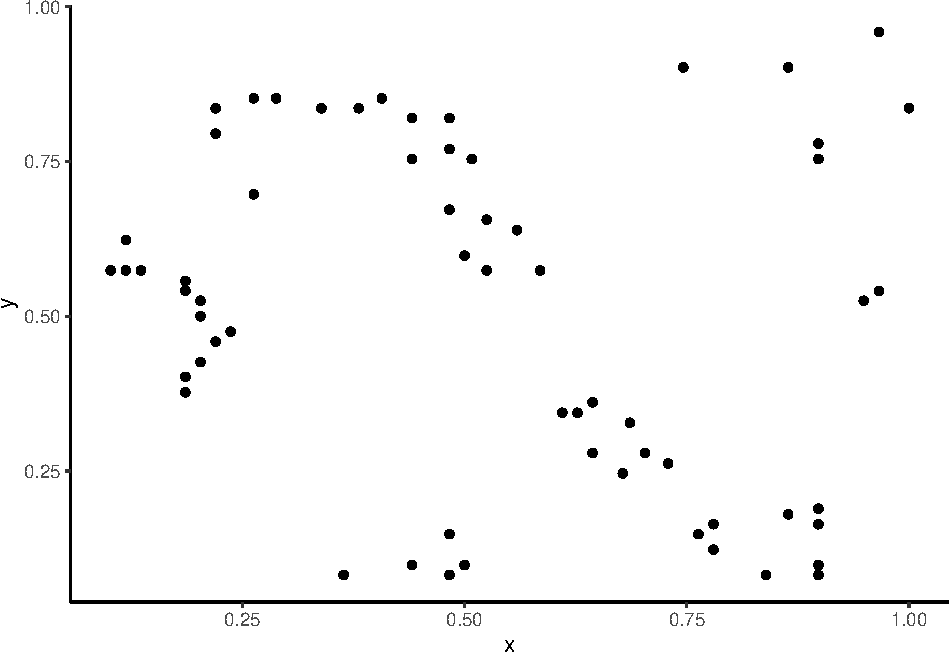
\includegraphics{project2_files/figure-latex/unnamed-chunk-1-1.pdf}
There seems to be some clusters of redwood. Want to fit an empirical
Neumann Scott Event-ref.

From the data there seems to be 8 mother nodes, with clusters of
redwoods around.

To avoid having to classify each point by hand, we use hierchical
clustering with L2 distance to find the cluster and their centers. We
use centroid clustering, and will use the centroids as estimation of
position to the mother node. We have already counted 8 mothernodes, so
we will use that estiamate.

\begin{Shaded}
\begin{Highlighting}[]
\CommentTok{# Doing hierchical clustering with centroid and eculidan}
\NormalTok{dist_mat <-}\StringTok{ }\KeywordTok{dist}\NormalTok{(redwood, }\DataTypeTok{method =} \StringTok{'euclidean'}\NormalTok{) }\CommentTok{# Calculate distances}
\NormalTok{hclust_centroid <-}\StringTok{ }\KeywordTok{hclust}\NormalTok{(dist_mat, }\DataTypeTok{method =} \StringTok{'centroid'}\NormalTok{) }\CommentTok{# Use centroid as moteher node}
\end{Highlighting}
\end{Shaded}

\begin{Shaded}
\begin{Highlighting}[]
\KeywordTok{plot}\NormalTok{(hclust_centroid, }\DataTypeTok{main =} \StringTok{"Cluster Dendogram for Redwoods. }\CharTok{\textbackslash{}n}\StringTok{ Centroid method w/ euclidian distance"}\NormalTok{)}
\end{Highlighting}
\end{Shaded}

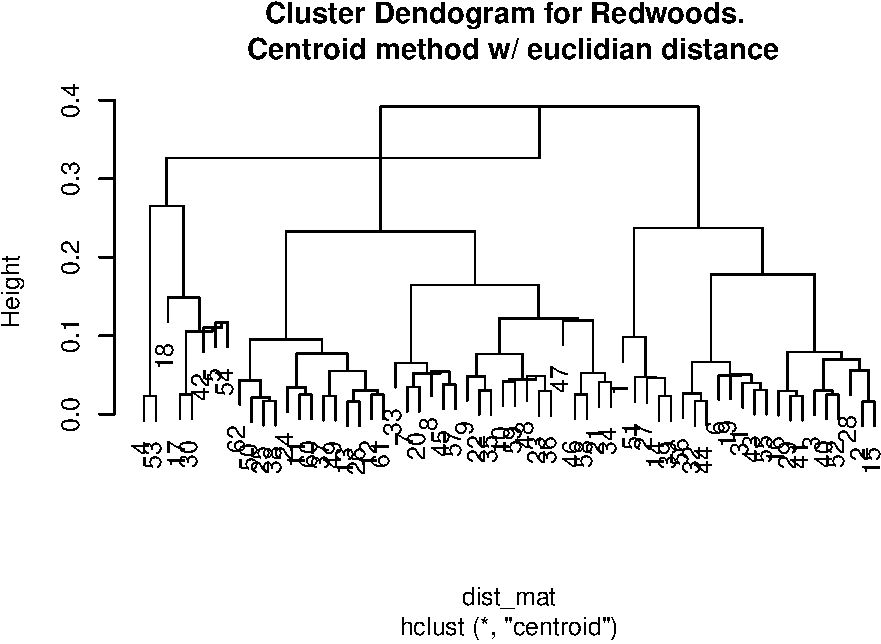
\includegraphics{project2_files/figure-latex/unnamed-chunk-3-1.pdf} The
cluster dendogram is illustrated in Figure \ref{some figure}

\begin{Shaded}
\begin{Highlighting}[]
\NormalTok{cut_centroid <-}\StringTok{ }\KeywordTok{cutree}\NormalTok{(hclust_centroid, }\DataTypeTok{k =} \DecValTok{8}\NormalTok{) }\CommentTok{# Find node of elements when we have 7 groups}
\end{Highlighting}
\end{Shaded}

\begin{Shaded}
\begin{Highlighting}[]
\NormalTok{redwood}\OperatorTok{$}\NormalTok{mother =}\StringTok{ }\KeywordTok{as.factor}\NormalTok{(cut_centroid)}
\end{Highlighting}
\end{Shaded}

\begin{Shaded}
\begin{Highlighting}[]
\KeywordTok{ggplot}\NormalTok{(redwood) }\OperatorTok{+}\StringTok{ }\KeywordTok{geom_point}\NormalTok{(}\KeywordTok{aes}\NormalTok{(}\DataTypeTok{x=}\NormalTok{ x, }\DataTypeTok{y =}\NormalTok{ y, }\DataTypeTok{color =}\NormalTok{ mother, }\DataTypeTok{shape =}\NormalTok{ mother)) }\OperatorTok{+}\StringTok{ }\KeywordTok{theme_classic}\NormalTok{() }\OperatorTok{+}\StringTok{  }\KeywordTok{scale_shape_manual}\NormalTok{(}\DataTypeTok{values=}\DecValTok{1}\OperatorTok{:}\KeywordTok{nlevels}\NormalTok{(redwood}\OperatorTok{$}\NormalTok{mother))}
\end{Highlighting}
\end{Shaded}

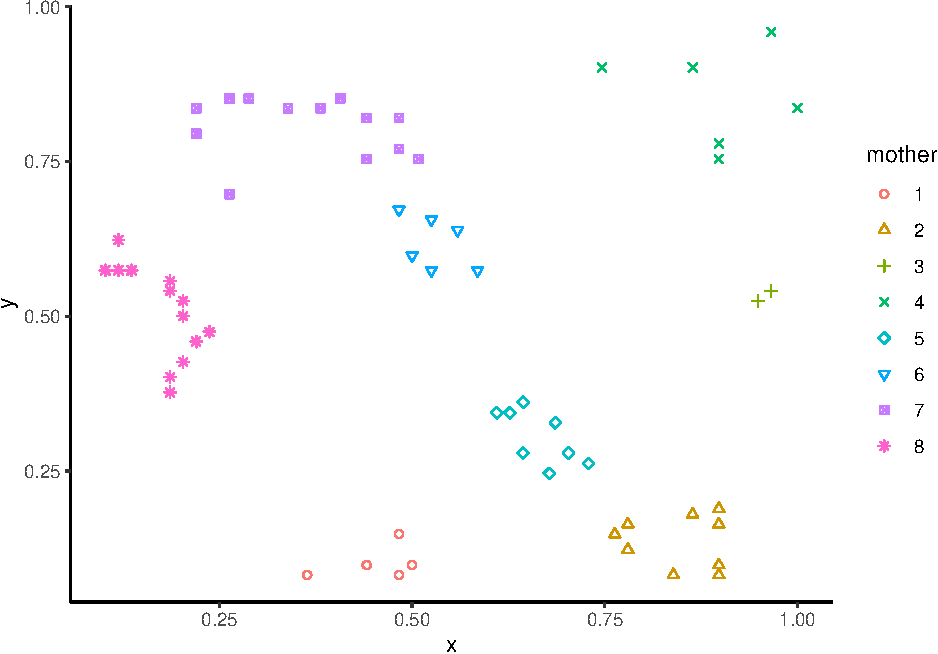
\includegraphics{project2_files/figure-latex/unnamed-chunk-6-1.pdf}

Classiying by cluster we get the following plot. See \ref{some figure}

We know find the position of the centroids. (As hclus does not give us
that we do it manually)

\begin{Shaded}
\begin{Highlighting}[]
\CommentTok{# Finding centers and count for each mother}
\NormalTok{mothers <-}\StringTok{ }\NormalTok{redwood }\OperatorTok\StringTok{ }
\StringTok{  }\KeywordTok{group_by}\NormalTok{(mother) }\OperatorTok\StringTok{ }
\StringTok{  }\KeywordTok{summarise}\NormalTok{(}\DataTypeTok{x =} \KeywordTok{mean}\NormalTok{(x),}
            \DataTypeTok{y =} \KeywordTok{mean}\NormalTok{(y), }
            \DataTypeTok{n =} \KeywordTok{n}\NormalTok{()) }\OperatorTok
\StringTok{  }\KeywordTok{as.data.frame}\NormalTok{()}
\end{Highlighting}
\end{Shaded}

We also want to estiamte the standard deviation. If we assume that each
cluster has independent standard deviation. And the each mother
estimation is unbiased. We get: (as deviation in x-coordinate and
y-coordiante are independent and equally normally distributed)

\begin{Shaded}
\begin{Highlighting}[]
\CommentTok{# Estimating standard dev }
\NormalTok{redwood_w_mother <-}\StringTok{ }\KeywordTok{left_join}\NormalTok{(redwood, mothers, }\DataTypeTok{by =} \KeywordTok{c}\NormalTok{(}\StringTok{"mother"}\NormalTok{))}
\KeywordTok{colnames}\NormalTok{(redwood_w_mother) <-}\StringTok{ }\KeywordTok{c}\NormalTok{(}\StringTok{"x"}\NormalTok{, }\StringTok{"y"}\NormalTok{, }\StringTok{"mother"}\NormalTok{, }\StringTok{"x.m"}\NormalTok{, }\StringTok{"y.m"}\NormalTok{, }\StringTok{"n"}\NormalTok{)}
\NormalTok{redwood_w_mother}\OperatorTok{$}\NormalTok{dist_mother <-}\StringTok{ }\KeywordTok{sqrt}\NormalTok{((redwood_w_mother}\OperatorTok{$}\NormalTok{x }\OperatorTok{-}\StringTok{ }\NormalTok{redwood_w_mother}\OperatorTok{$}\NormalTok{x.m)}\OperatorTok{^}\DecValTok{2} \OperatorTok{+}\StringTok{ }\NormalTok{(redwood_w_mother}\OperatorTok{$}\NormalTok{y }\OperatorTok{-}\StringTok{ }\NormalTok{redwood_w_mother}\OperatorTok{$}\NormalTok{y.m)}\OperatorTok{^}\DecValTok{2}\NormalTok{)}
\NormalTok{redwood_w_mother}\OperatorTok{$}\NormalTok{x.dist <-}\StringTok{ }\NormalTok{redwood_w_mother}\OperatorTok{$}\NormalTok{x }\OperatorTok{-}\StringTok{ }\NormalTok{redwood_w_mother}\OperatorTok{$}\NormalTok{x.m}
\NormalTok{redwood_w_mother}\OperatorTok{$}\NormalTok{y.dist <-}\StringTok{ }\NormalTok{redwood_w_mother}\OperatorTok{$}\NormalTok{y }\OperatorTok{-}\StringTok{ }\NormalTok{redwood_w_mother}\OperatorTok{$}\NormalTok{y.m}

\NormalTok{std2 <-}\StringTok{ }\DecValTok{1}\OperatorTok{/}\NormalTok{(}\KeywordTok{length}\NormalTok{(redwood_w_mother}\OperatorTok{$}\NormalTok{x.dist) }\OperatorTok{+}\StringTok{ }\KeywordTok{length}\NormalTok{(redwood_w_mother}\OperatorTok{$}\NormalTok{y.dist) }\OperatorTok{-}\StringTok{ }\DecValTok{1}\NormalTok{)}\OperatorTok{*}\StringTok{ }\NormalTok{(}\KeywordTok{sum}\NormalTok{(redwood_w_mother}\OperatorTok{$}\NormalTok{x.dist}\OperatorTok{^}\DecValTok{2}\NormalTok{) }\OperatorTok{+}\StringTok{ }\KeywordTok{sum}\NormalTok{(redwood_w_mother}\OperatorTok{$}\NormalTok{y.dist}\OperatorTok{^}\DecValTok{2}\NormalTok{))}

\NormalTok{q95 <-}\StringTok{ }\KeywordTok{qnorm}\NormalTok{(}\FloatTok{0.95}\NormalTok{, }\DataTypeTok{mean =} \DecValTok{0}\NormalTok{, }\DataTypeTok{sd =} \KeywordTok{sqrt}\NormalTok{(std2))}
\end{Highlighting}
\end{Shaded}

If we assume that they a common standard deviation we get: 0.0033968

Plotting the redwood forest, with the mother nodes we get:

\begin{Shaded}
\begin{Highlighting}[]
\KeywordTok{ggplot}\NormalTok{() }\OperatorTok{+}
\StringTok{  }\KeywordTok{geom_point}\NormalTok{(}\KeywordTok{aes}\NormalTok{(}\DataTypeTok{x=}\NormalTok{ redwood}\OperatorTok{$}\NormalTok{x, }\DataTypeTok{y =}\NormalTok{ redwood}\OperatorTok{$}\NormalTok{y, }\DataTypeTok{color =}\NormalTok{ redwood}\OperatorTok{$}\NormalTok{mother, }\DataTypeTok{shape =}\NormalTok{ redwood}\OperatorTok{$}\NormalTok{mother)) }\OperatorTok{+}
\StringTok{  }\KeywordTok{theme_classic}\NormalTok{() }\OperatorTok{+}\StringTok{ }
\StringTok{  }\KeywordTok{scale_shape_manual}\NormalTok{(}\DataTypeTok{values=}\DecValTok{1}\OperatorTok{:}\KeywordTok{nlevels}\NormalTok{(redwood}\OperatorTok{$}\NormalTok{mother)) }\OperatorTok{+}
\StringTok{  }\KeywordTok{geom_point}\NormalTok{(}\KeywordTok{aes}\NormalTok{(}\DataTypeTok{x =}\NormalTok{ mothers}\OperatorTok{$}\NormalTok{x, }\DataTypeTok{y =}\NormalTok{ mothers}\OperatorTok{$}\NormalTok{y)) }\OperatorTok{+}\StringTok{ }
\StringTok{  }\KeywordTok{geom_circle}\NormalTok{(}\KeywordTok{aes}\NormalTok{(}\DataTypeTok{r =} \KeywordTok{rep}\NormalTok{(q95, }\KeywordTok{length}\NormalTok{(mothers}\OperatorTok{$}\NormalTok{y)), }\DataTypeTok{y0 =}\NormalTok{ mothers}\OperatorTok{$}\NormalTok{y, }\DataTypeTok{x0 =}\NormalTok{ mothers}\OperatorTok{$}\NormalTok{x), }\DataTypeTok{linetype =} \StringTok{"dashed"}\NormalTok{, }\DataTypeTok{alpha =} \FloatTok{0.8}\NormalTok{)}
\end{Highlighting}
\end{Shaded}

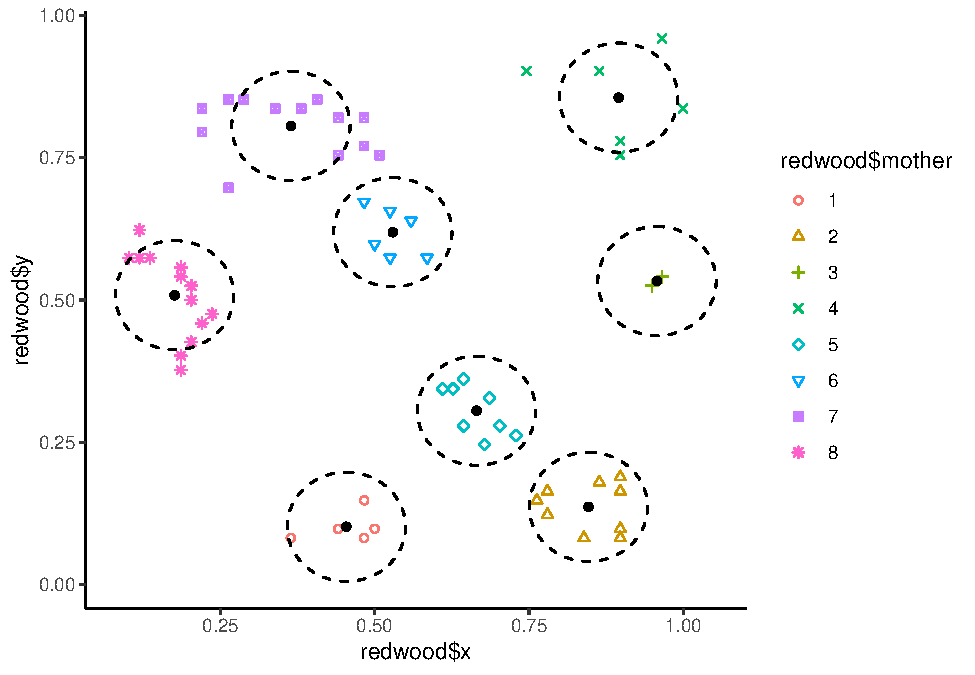
\includegraphics{project2_files/figure-latex/unnamed-chunk-9-1.pdf}

\begin{Shaded}
\begin{Highlighting}[]
\CommentTok{# Mean of realization around mother}
\NormalTok{ns <-}\StringTok{ }\NormalTok{redwood }\OperatorTok\StringTok{ }\KeywordTok{group_by}\NormalTok{(mother) }\OperatorTok\StringTok{ }\KeywordTok{summarise}\NormalTok{(}\DataTypeTok{n =} \KeywordTok{n}\NormalTok{()) }\OperatorTok\StringTok{ }\KeywordTok{ungroup}\NormalTok{()}
\NormalTok{lambda.c <-}\StringTok{ }\KeywordTok{mean}\NormalTok{(ns}\OperatorTok{$}\NormalTok{n)}
\end{Highlighting}
\end{Shaded}

TODO: Q are mother nodes a part of the count ? TODO: Q what is the
TORUS-3d algorithm not in my version of the note (p.~131). Is it to
project outliers onto some torus? Then shifting them around some

So the parameters of our model are:

\begin{itemize}
\item
  Poisson with \(lambda = 8\) for number of mother nodes
\item
  \(\sigma^2_c\) = 0.0033968
\item
  Poisson behind number of childrean with \$lambda = \$7.75
\item
  Gaussian spread around mother node
\end{itemize}

\begin{Shaded}
\begin{Highlighting}[]
\CommentTok{# ppinit does not seem to read properly so we do it manually}
\CommentTok{# redwood.pp <- ppinit("redwood.dat")}
\CommentTok{# plot(Kfn(redwood.pp, 1, k = 200), type="b", xlab="distance", ylab="L(t)")}
\end{Highlighting}
\end{Shaded}

\begin{Shaded}
\begin{Highlighting}[]
\NormalTok{redwood <-}\StringTok{ }\KeywordTok{read.csv}\NormalTok{(}\StringTok{"redwood.dat"}\NormalTok{, }\DataTypeTok{header =}\NormalTok{ F, }\DataTypeTok{sep =} \StringTok{" "}\NormalTok{)}
\NormalTok{redwood <-}\StringTok{ }\KeywordTok{as.data.frame}\NormalTok{(redwood)}
\KeywordTok{colnames}\NormalTok{(redwood) <-}\StringTok{ }\KeywordTok{c}\NormalTok{(}\StringTok{"x"}\NormalTok{, }\StringTok{"y"}\NormalTok{)}

\NormalTok{D =}\StringTok{ }\KeywordTok{ppregion}\NormalTok{(}\DataTypeTok{xl =} \DecValTok{0}\NormalTok{, }\DataTypeTok{xu =} \DecValTok{1}\NormalTok{, }\DataTypeTok{yl =} \DecValTok{0}\NormalTok{, }\DataTypeTok{yu =} \DecValTok{1}\NormalTok{)}

\NormalTok{redwood.pp2 <-}\StringTok{ }\KeywordTok{list}\NormalTok{(}
  \DataTypeTok{x =}\NormalTok{ redwood}\OperatorTok{$}\NormalTok{x, }
  \DataTypeTok{y =}\NormalTok{ redwood}\OperatorTok{$}\NormalTok{y, }
  \DataTypeTok{area =}\NormalTok{ D}
\NormalTok{)}


\NormalTok{kfn <-}\StringTok{ }\KeywordTok{Kfn}\NormalTok{(redwood.pp2, }\DecValTok{1}\NormalTok{, }\DataTypeTok{k =} \DecValTok{200}\NormalTok{)}
\KeywordTok{plot}\NormalTok{(kfn, }\DataTypeTok{type=}\StringTok{"b"}\NormalTok{, }\DataTypeTok{xlab=}\StringTok{"distance"}\NormalTok{, }\DataTypeTok{ylab=}\StringTok{"L(t)"}\NormalTok{)}
\end{Highlighting}
\end{Shaded}

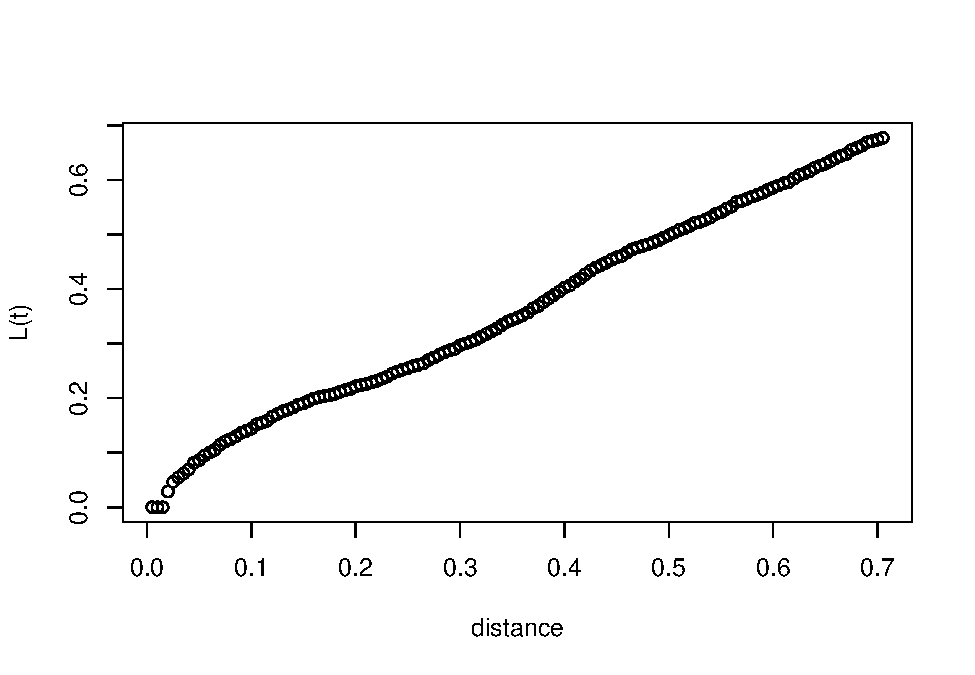
\includegraphics{project2_files/figure-latex/unnamed-chunk-12-1.pdf}

\begin{Shaded}
\begin{Highlighting}[]
\CommentTok{# Distances we want to check out }
\NormalTok{neumann_scot_generate <-}\StringTok{ }\ControlFlowTok{function}\NormalTok{(lambda.m, lambda.c, std2, seed)\{}
  \KeywordTok{set.seed}\NormalTok{(seed)}
\NormalTok{  count =}\StringTok{ }\DecValTok{0}
\NormalTok{  k <-}\StringTok{ }\KeywordTok{rpois}\NormalTok{(}\DataTypeTok{n =} \DecValTok{1}\NormalTok{, }\DataTypeTok{lambda =}\NormalTok{ lambda.m)}
\NormalTok{  xs <-}\StringTok{ }\KeywordTok{c}\NormalTok{()}
\NormalTok{  mothers <-}\StringTok{ }\KeywordTok{c}\NormalTok{()}
  \ControlFlowTok{for}\NormalTok{(j }\ControlFlowTok{in} \DecValTok{1}\OperatorTok{:}\NormalTok{k)\{}
\NormalTok{    xj <-}\StringTok{ }\KeywordTok{runif}\NormalTok{(}\DecValTok{2}\NormalTok{)}
\NormalTok{    n.child <-}\StringTok{ }\KeywordTok{rpois}\NormalTok{(}\DecValTok{1}\NormalTok{, }\DataTypeTok{lambda =}\NormalTok{ lambda.c)}
    \ControlFlowTok{for}\NormalTok{(i }\ControlFlowTok{in} \DecValTok{1}\OperatorTok{:}\NormalTok{n.child)\{}
\NormalTok{      x <-}\StringTok{ }\NormalTok{MASS}\OperatorTok{::}\KeywordTok{mvrnorm}\NormalTok{(}\DataTypeTok{n =} \DecValTok{1}\NormalTok{, }\DataTypeTok{Sigma =}\NormalTok{ std2}\OperatorTok{*}\KeywordTok{diag}\NormalTok{(}\DecValTok{2}\NormalTok{), }\DataTypeTok{mu =}\NormalTok{ xj)}
      \CommentTok{# Just project for now}
      \ControlFlowTok{if}\NormalTok{(x[}\DecValTok{1}\NormalTok{] }\OperatorTok{<}\StringTok{ }\DecValTok{0}\NormalTok{) x[}\DecValTok{1}\NormalTok{] <-}\StringTok{ }\DecValTok{0} 
      \ControlFlowTok{if}\NormalTok{(x[}\DecValTok{1}\NormalTok{] }\OperatorTok{>}\StringTok{ }\DecValTok{1}\NormalTok{) x[}\DecValTok{1}\NormalTok{] <-}\StringTok{ }\DecValTok{1}
      
      \ControlFlowTok{if}\NormalTok{(x[}\DecValTok{2}\NormalTok{] }\OperatorTok{<}\StringTok{ }\DecValTok{0}\NormalTok{) x[}\DecValTok{2}\NormalTok{] <-}\StringTok{ }\DecValTok{0} 
      \ControlFlowTok{if}\NormalTok{(x[}\DecValTok{2}\NormalTok{] }\OperatorTok{>}\StringTok{ }\DecValTok{1}\NormalTok{) x[}\DecValTok{2}\NormalTok{] <-}\StringTok{ }\DecValTok{1}
\NormalTok{      xs <-}\StringTok{ }\KeywordTok{rbind}\NormalTok{(xs, x)}
\NormalTok{    \}}
\NormalTok{    count <-}\StringTok{ }\NormalTok{count }\OperatorTok{+}\StringTok{ }\NormalTok{n.child}
\NormalTok{    mothers <-}\StringTok{ }\KeywordTok{c}\NormalTok{(mothers, }\KeywordTok{rep}\NormalTok{(j, n.child))}
\NormalTok{  \}}
  \KeywordTok{list}\NormalTok{(}\DataTypeTok{xs =}\NormalTok{ xs, }\DataTypeTok{mothers =}\NormalTok{ mothers) }
\NormalTok{\}}

\NormalTok{lambda.m <-}\StringTok{ }\DecValTok{8}
\NormalTok{n.rels <-}\StringTok{ }\DecValTok{1000}
\NormalTok{rels <-}\StringTok{ }\KeywordTok{lapply}\NormalTok{(}\DecValTok{1}\OperatorTok{:}\NormalTok{n.rels, }\ControlFlowTok{function}\NormalTok{(seed) }\KeywordTok{neumann_scot_generate}\NormalTok{(}\DataTypeTok{lambda.m =}\NormalTok{ lambda.m, }\DataTypeTok{lambda.c =}\NormalTok{ lambda.c, }\DataTypeTok{std2 =}\NormalTok{ std2, }\DataTypeTok{seed =}\NormalTok{ seed)}\OperatorTok{$}\NormalTok{xs)}
\NormalTok{rels <-}\StringTok{ }\KeywordTok{lapply}\NormalTok{(rels, }\ControlFlowTok{function}\NormalTok{(rel) }\KeywordTok{list}\NormalTok{(}\DataTypeTok{x =}\NormalTok{ rel[,}\DecValTok{1}\NormalTok{], }\DataTypeTok{y =}\NormalTok{ rel[,}\DecValTok{2}\NormalTok{], }\DataTypeTok{area =}\NormalTok{ D))}
\NormalTok{kfns <-}\StringTok{ }\KeywordTok{lapply}\NormalTok{(rels, }\ControlFlowTok{function}\NormalTok{(rel) }\KeywordTok{Kfn}\NormalTok{(rel, }\DecValTok{1}\NormalTok{, }\DataTypeTok{k =} \DecValTok{200}\NormalTok{))}
\NormalTok{bands <-}\StringTok{ }\KeywordTok{sapply}\NormalTok{(kfns, }\ControlFlowTok{function}\NormalTok{(kfn) kfn}\OperatorTok{$}\NormalTok{y)}
\NormalTok{lower_band <-}\StringTok{ }\KeywordTok{apply}\NormalTok{(bands, }\DecValTok{1}\NormalTok{, }\ControlFlowTok{function}\NormalTok{(x) }\KeywordTok{quantile}\NormalTok{(x, }\DataTypeTok{probs =} \FloatTok{0.025}\NormalTok{))}
\NormalTok{upper_band <-}\StringTok{ }\KeywordTok{apply}\NormalTok{(bands, }\DecValTok{1}\NormalTok{, }\ControlFlowTok{function}\NormalTok{(x) }\KeywordTok{quantile}\NormalTok{(x, }\DataTypeTok{probs =} \FloatTok{0.975}\NormalTok{))}
\NormalTok{mid_band <-}\StringTok{ }\KeywordTok{apply}\NormalTok{(bands, }\DecValTok{1}\NormalTok{, }\ControlFlowTok{function}\NormalTok{(x) }\KeywordTok{quantile}\NormalTok{(x, }\DataTypeTok{probs =} \FloatTok{0.5}\NormalTok{))}

\KeywordTok{ggplot}\NormalTok{() }\OperatorTok{+}\StringTok{ }\KeywordTok{geom_ribbon}\NormalTok{(}\KeywordTok{aes}\NormalTok{(}\DataTypeTok{x =}\NormalTok{ kfn}\OperatorTok{$}\NormalTok{x, }\DataTypeTok{ymax =}\NormalTok{ upper_band, }\DataTypeTok{ymin =}\NormalTok{ lower_band), }\DataTypeTok{alpha =} \FloatTok{0.3}\NormalTok{) }\OperatorTok{+}\StringTok{ }\KeywordTok{geom_line}\NormalTok{(}\KeywordTok{aes}\NormalTok{(}\DataTypeTok{x =}\NormalTok{ kfn}\OperatorTok{$}\NormalTok{x, }\DataTypeTok{y =}\NormalTok{ kfn}\OperatorTok{$}\NormalTok{y))}
\end{Highlighting}
\end{Shaded}

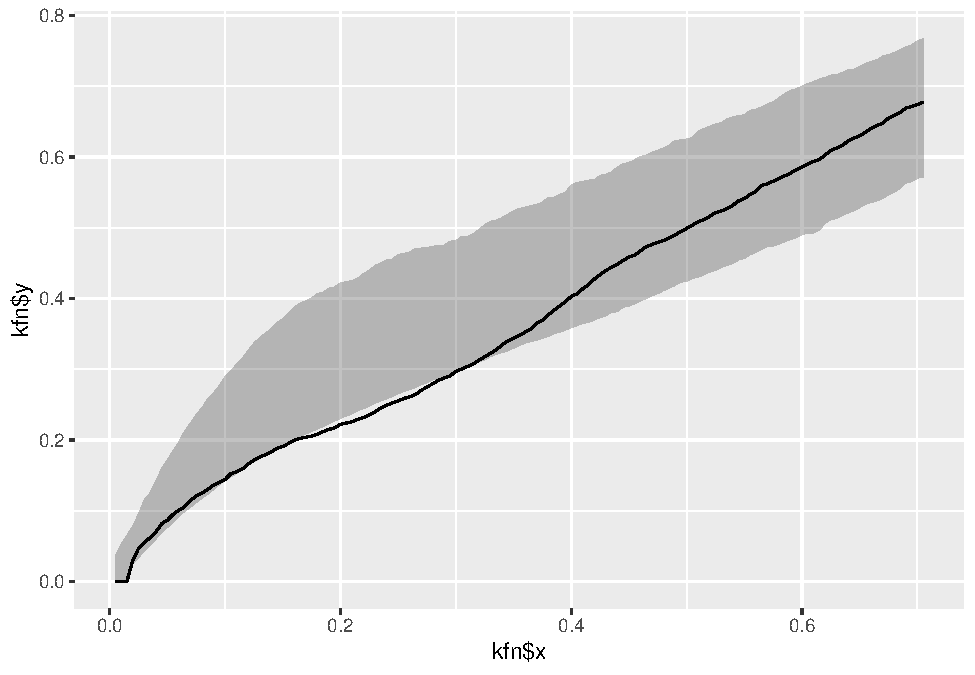
\includegraphics{project2_files/figure-latex/unnamed-chunk-13-1.pdf}

Seems to be a bit bad a mid distances, a higher variance might on spread
might help on that.

\begin{Shaded}
\begin{Highlighting}[]
\NormalTok{lambda.m <-}\StringTok{ }\DecValTok{8}
\NormalTok{n.rels <-}\StringTok{ }\DecValTok{1000}
\NormalTok{std2 <-}\StringTok{ }\NormalTok{std2}\OperatorTok{*}\DecValTok{4}
\NormalTok{rels <-}\StringTok{ }\KeywordTok{lapply}\NormalTok{(}\DecValTok{1}\OperatorTok{:}\NormalTok{n.rels, }\ControlFlowTok{function}\NormalTok{(seed) }\KeywordTok{neumann_scot_generate}\NormalTok{(}\DataTypeTok{lambda.m =}\NormalTok{ lambda.m, }\DataTypeTok{lambda.c =}\NormalTok{ lambda.c, }\DataTypeTok{std2 =}\NormalTok{ std2, }\DataTypeTok{seed =}\NormalTok{ seed)}\OperatorTok{$}\NormalTok{xs)}
\NormalTok{rels <-}\StringTok{ }\KeywordTok{lapply}\NormalTok{(rels, }\ControlFlowTok{function}\NormalTok{(rel) }\KeywordTok{list}\NormalTok{(}\DataTypeTok{x =}\NormalTok{ rel[,}\DecValTok{1}\NormalTok{], }\DataTypeTok{y =}\NormalTok{ rel[,}\DecValTok{2}\NormalTok{], }\DataTypeTok{area =}\NormalTok{ D))}
\NormalTok{kfns <-}\StringTok{ }\KeywordTok{lapply}\NormalTok{(rels, }\ControlFlowTok{function}\NormalTok{(rel) }\KeywordTok{Kfn}\NormalTok{(rel, }\DecValTok{1}\NormalTok{, }\DataTypeTok{k =} \DecValTok{200}\NormalTok{))}
\NormalTok{bands <-}\StringTok{ }\KeywordTok{sapply}\NormalTok{(kfns, }\ControlFlowTok{function}\NormalTok{(kfn) kfn}\OperatorTok{$}\NormalTok{y)}
\NormalTok{lower_band <-}\StringTok{ }\KeywordTok{apply}\NormalTok{(bands, }\DecValTok{1}\NormalTok{, }\ControlFlowTok{function}\NormalTok{(x) }\KeywordTok{quantile}\NormalTok{(x, }\DataTypeTok{probs =} \FloatTok{0.025}\NormalTok{))}
\NormalTok{upper_band <-}\StringTok{ }\KeywordTok{apply}\NormalTok{(bands, }\DecValTok{1}\NormalTok{, }\ControlFlowTok{function}\NormalTok{(x) }\KeywordTok{quantile}\NormalTok{(x, }\DataTypeTok{probs =} \FloatTok{0.975}\NormalTok{))}
\NormalTok{mid_band <-}\StringTok{ }\KeywordTok{apply}\NormalTok{(bands, }\DecValTok{1}\NormalTok{, }\ControlFlowTok{function}\NormalTok{(x) }\KeywordTok{quantile}\NormalTok{(x, }\DataTypeTok{probs =} \FloatTok{0.5}\NormalTok{))}

\KeywordTok{ggplot}\NormalTok{() }\OperatorTok{+}\StringTok{ }\KeywordTok{geom_ribbon}\NormalTok{(}\KeywordTok{aes}\NormalTok{(}\DataTypeTok{x =}\NormalTok{ kfn}\OperatorTok{$}\NormalTok{x, }\DataTypeTok{ymax =}\NormalTok{ upper_band, }\DataTypeTok{ymin =}\NormalTok{ lower_band), }\DataTypeTok{alpha =} \FloatTok{0.3}\NormalTok{) }\OperatorTok{+}\StringTok{ }\KeywordTok{geom_line}\NormalTok{(}\KeywordTok{aes}\NormalTok{(}\DataTypeTok{x =}\NormalTok{ kfn}\OperatorTok{$}\NormalTok{x, }\DataTypeTok{y =}\NormalTok{ kfn}\OperatorTok{$}\NormalTok{y))}
\end{Highlighting}
\end{Shaded}

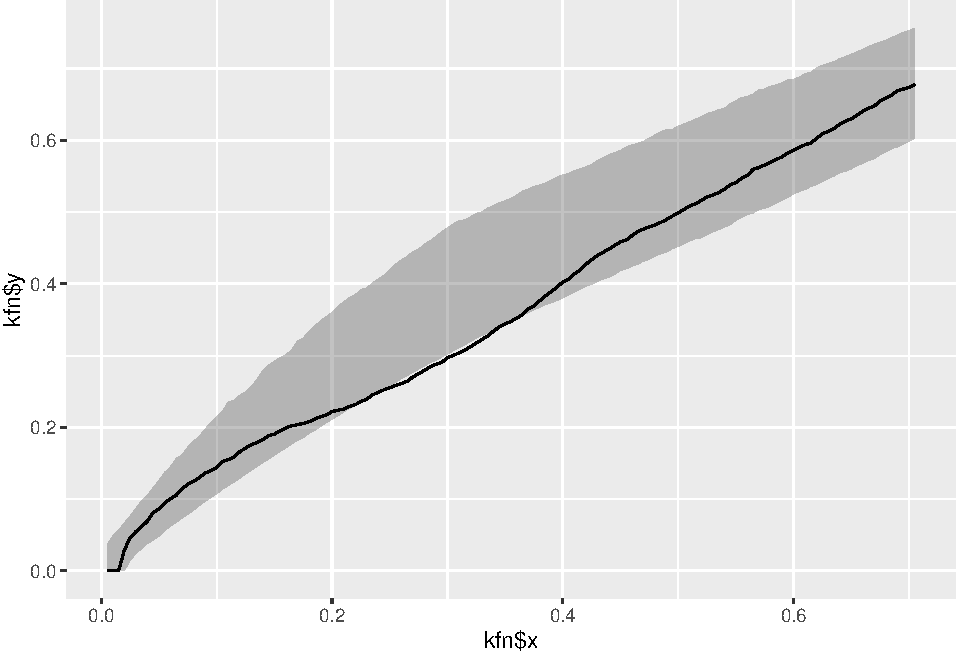
\includegraphics{project2_files/figure-latex/unnamed-chunk-14-1.pdf}

Helped somewhat, change lambda somewhat to see if it helps.

\begin{Shaded}
\begin{Highlighting}[]
\NormalTok{lambda.m <-}\StringTok{ }\FloatTok{9.5}
\NormalTok{n.rels <-}\StringTok{ }\DecValTok{1000}
\NormalTok{std2 <-}\StringTok{ }\NormalTok{std2}
\NormalTok{rels <-}\StringTok{ }\KeywordTok{lapply}\NormalTok{(}\DecValTok{1}\OperatorTok{:}\NormalTok{n.rels, }\ControlFlowTok{function}\NormalTok{(seed) }\KeywordTok{neumann_scot_generate}\NormalTok{(}\DataTypeTok{lambda.m =}\NormalTok{ lambda.m, }\DataTypeTok{lambda.c =}\NormalTok{ lambda.c, }\DataTypeTok{std2 =}\NormalTok{ std2, }\DataTypeTok{seed =}\NormalTok{ seed)}\OperatorTok{$}\NormalTok{xs)}
\NormalTok{rels <-}\StringTok{ }\KeywordTok{lapply}\NormalTok{(rels, }\ControlFlowTok{function}\NormalTok{(rel) }\KeywordTok{list}\NormalTok{(}\DataTypeTok{x =}\NormalTok{ rel[,}\DecValTok{1}\NormalTok{], }\DataTypeTok{y =}\NormalTok{ rel[,}\DecValTok{2}\NormalTok{], }\DataTypeTok{area =}\NormalTok{ D))}
\NormalTok{kfns <-}\StringTok{ }\KeywordTok{lapply}\NormalTok{(rels, }\ControlFlowTok{function}\NormalTok{(rel) }\KeywordTok{Kfn}\NormalTok{(rel, }\DecValTok{1}\NormalTok{, }\DataTypeTok{k =} \DecValTok{200}\NormalTok{))}
\NormalTok{bands <-}\StringTok{ }\KeywordTok{sapply}\NormalTok{(kfns, }\ControlFlowTok{function}\NormalTok{(kfn) kfn}\OperatorTok{$}\NormalTok{y)}
\NormalTok{lower_band <-}\StringTok{ }\KeywordTok{apply}\NormalTok{(bands, }\DecValTok{1}\NormalTok{, }\ControlFlowTok{function}\NormalTok{(x) }\KeywordTok{quantile}\NormalTok{(x, }\DataTypeTok{probs =} \FloatTok{0.025}\NormalTok{))}
\NormalTok{upper_band <-}\StringTok{ }\KeywordTok{apply}\NormalTok{(bands, }\DecValTok{1}\NormalTok{, }\ControlFlowTok{function}\NormalTok{(x) }\KeywordTok{quantile}\NormalTok{(x, }\DataTypeTok{probs =} \FloatTok{0.975}\NormalTok{))}
\NormalTok{mid_band <-}\StringTok{ }\KeywordTok{apply}\NormalTok{(bands, }\DecValTok{1}\NormalTok{, }\ControlFlowTok{function}\NormalTok{(x) }\KeywordTok{quantile}\NormalTok{(x, }\DataTypeTok{probs =} \FloatTok{0.5}\NormalTok{))}

\KeywordTok{ggplot}\NormalTok{() }\OperatorTok{+}\StringTok{ }\KeywordTok{geom_ribbon}\NormalTok{(}\KeywordTok{aes}\NormalTok{(}\DataTypeTok{x =}\NormalTok{ kfn}\OperatorTok{$}\NormalTok{x, }\DataTypeTok{ymax =}\NormalTok{ upper_band, }\DataTypeTok{ymin =}\NormalTok{ lower_band), }\DataTypeTok{alpha =} \FloatTok{0.3}\NormalTok{) }\OperatorTok{+}\StringTok{ }\KeywordTok{geom_line}\NormalTok{(}\KeywordTok{aes}\NormalTok{(}\DataTypeTok{x =}\NormalTok{ kfn}\OperatorTok{$}\NormalTok{x, }\DataTypeTok{y =}\NormalTok{ kfn}\OperatorTok{$}\NormalTok{y))}
\end{Highlighting}
\end{Shaded}

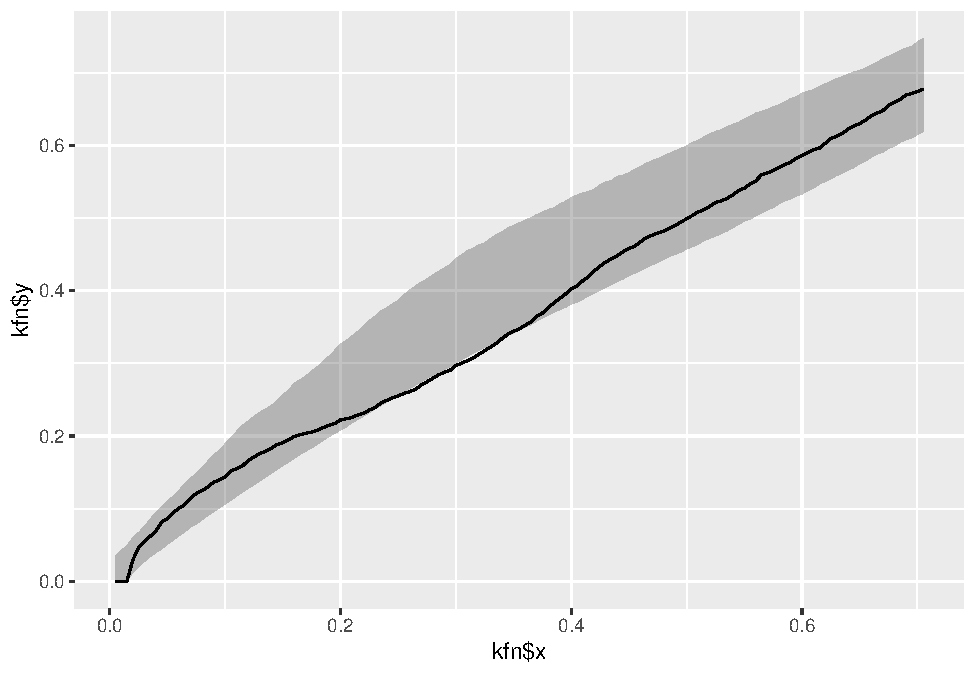
\includegraphics{project2_files/figure-latex/unnamed-chunk-15-1.pdf}
Does not seem to have any good effect. We try to increase variance
again.

\begin{Shaded}
\begin{Highlighting}[]
\NormalTok{lambda.m <-}\StringTok{ }\DecValTok{8}
\NormalTok{n.rels <-}\StringTok{ }\DecValTok{1000}
\NormalTok{std2 <-}\StringTok{ }\NormalTok{std2}\OperatorTok{*}\DecValTok{4}
\NormalTok{rels <-}\StringTok{ }\KeywordTok{lapply}\NormalTok{(}\DecValTok{1}\OperatorTok{:}\NormalTok{n.rels, }\ControlFlowTok{function}\NormalTok{(seed) }\KeywordTok{neumann_scot_generate}\NormalTok{(}\DataTypeTok{lambda.m =}\NormalTok{ lambda.m, }\DataTypeTok{lambda.c =}\NormalTok{ lambda.c, }\DataTypeTok{std2 =}\NormalTok{ std2, }\DataTypeTok{seed =}\NormalTok{ seed)}\OperatorTok{$}\NormalTok{xs)}
\NormalTok{rels <-}\StringTok{ }\KeywordTok{lapply}\NormalTok{(rels, }\ControlFlowTok{function}\NormalTok{(rel) }\KeywordTok{list}\NormalTok{(}\DataTypeTok{x =}\NormalTok{ rel[,}\DecValTok{1}\NormalTok{], }\DataTypeTok{y =}\NormalTok{ rel[,}\DecValTok{2}\NormalTok{], }\DataTypeTok{area =}\NormalTok{ D))}
\NormalTok{kfns <-}\StringTok{ }\KeywordTok{lapply}\NormalTok{(rels, }\ControlFlowTok{function}\NormalTok{(rel) }\KeywordTok{Kfn}\NormalTok{(rel, }\DecValTok{1}\NormalTok{, }\DataTypeTok{k =} \DecValTok{200}\NormalTok{))}
\NormalTok{bands <-}\StringTok{ }\KeywordTok{sapply}\NormalTok{(kfns, }\ControlFlowTok{function}\NormalTok{(kfn) kfn}\OperatorTok{$}\NormalTok{y)}
\NormalTok{lower_band <-}\StringTok{ }\KeywordTok{apply}\NormalTok{(bands, }\DecValTok{1}\NormalTok{, }\ControlFlowTok{function}\NormalTok{(x) }\KeywordTok{quantile}\NormalTok{(x, }\DataTypeTok{probs =} \FloatTok{0.025}\NormalTok{))}
\NormalTok{upper_band <-}\StringTok{ }\KeywordTok{apply}\NormalTok{(bands, }\DecValTok{1}\NormalTok{, }\ControlFlowTok{function}\NormalTok{(x) }\KeywordTok{quantile}\NormalTok{(x, }\DataTypeTok{probs =} \FloatTok{0.975}\NormalTok{))}
\NormalTok{mid_band <-}\StringTok{ }\KeywordTok{apply}\NormalTok{(bands, }\DecValTok{1}\NormalTok{, }\ControlFlowTok{function}\NormalTok{(x) }\KeywordTok{quantile}\NormalTok{(x, }\DataTypeTok{probs =} \FloatTok{0.5}\NormalTok{))}

\KeywordTok{ggplot}\NormalTok{() }\OperatorTok{+}\StringTok{ }\KeywordTok{geom_ribbon}\NormalTok{(}\KeywordTok{aes}\NormalTok{(}\DataTypeTok{x =}\NormalTok{ kfn}\OperatorTok{$}\NormalTok{x, }\DataTypeTok{ymax =}\NormalTok{ upper_band, }\DataTypeTok{ymin =}\NormalTok{ lower_band), }\DataTypeTok{alpha =} \FloatTok{0.3}\NormalTok{) }\OperatorTok{+}\StringTok{ }\KeywordTok{geom_line}\NormalTok{(}\KeywordTok{aes}\NormalTok{(}\DataTypeTok{x =}\NormalTok{ kfn}\OperatorTok{$}\NormalTok{x, }\DataTypeTok{y =}\NormalTok{ kfn}\OperatorTok{$}\NormalTok{y))}
\end{Highlighting}
\end{Shaded}

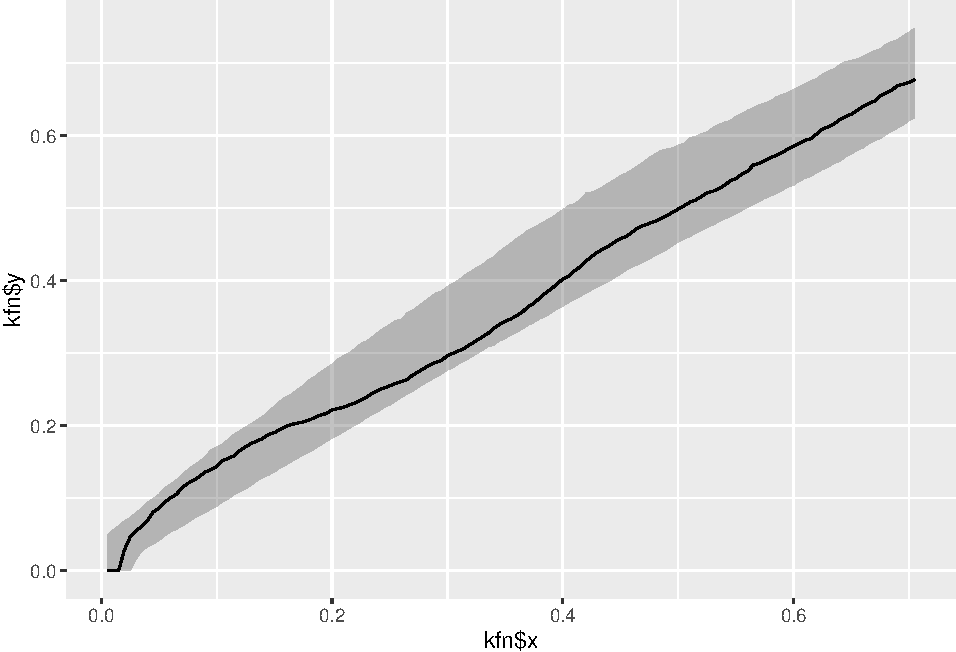
\includegraphics{project2_files/figure-latex/unnamed-chunk-16-1.pdf}
Realization is now within 95\% confidence interval an we har happy with
the fit. Ended up using

\begin{itemize}
\item
  Poisson with \(lambda = 8\) for number of mother nodes
\item
  \(\sigma^2_c\) = 0.0543488
\item
  Poisson behind number of childrean with \$lambda = \$7.75
\item
  Gaussian spread around mother node
\end{itemize}

Display three realiations of the model with this parameters to what was
observed (we overlay our grouping to the plots) :

\begin{Shaded}
\begin{Highlighting}[]
\NormalTok{df1 <-}\StringTok{ }\KeywordTok{neumann_scot_generate}\NormalTok{(}\DataTypeTok{lambda.m =}\NormalTok{ lambda.m, }\DataTypeTok{lambda.c =}\NormalTok{ lambda.c, }\DataTypeTok{std2 =}\NormalTok{ std2, }\DataTypeTok{seed =} \DecValTok{1}\NormalTok{)}
\NormalTok{df1 <-}\StringTok{ }\KeywordTok{as.data.frame}\NormalTok{(df1)}
\KeywordTok{colnames}\NormalTok{(df1) <-}\StringTok{ }\KeywordTok{c}\NormalTok{(}\StringTok{"x"}\NormalTok{, }\StringTok{"y"}\NormalTok{, }\StringTok{"mothers"}\NormalTok{)}
\NormalTok{df1}\OperatorTok{$}\NormalTok{mothers <-}\StringTok{ }\KeywordTok{as.factor}\NormalTok{(df1}\OperatorTok{$}\NormalTok{mothers)}
\NormalTok{df2 <-}\StringTok{ }\KeywordTok{neumann_scot_generate}\NormalTok{(}\DataTypeTok{lambda.m =}\NormalTok{ lambda.m, }\DataTypeTok{lambda.c =}\NormalTok{ lambda.c, }\DataTypeTok{std2 =}\NormalTok{ std2, }\DataTypeTok{seed =} \DecValTok{2}\NormalTok{)}
\NormalTok{df2 <-}\StringTok{ }\KeywordTok{as.data.frame}\NormalTok{(df2)}
\KeywordTok{colnames}\NormalTok{(df2) <-}\StringTok{ }\KeywordTok{c}\NormalTok{(}\StringTok{"x"}\NormalTok{, }\StringTok{"y"}\NormalTok{, }\StringTok{"mothers"}\NormalTok{)}
\NormalTok{df2}\OperatorTok{$}\NormalTok{mothers <-}\StringTok{ }\KeywordTok{as.factor}\NormalTok{(df2}\OperatorTok{$}\NormalTok{mothers)}
\NormalTok{df3 <-}\StringTok{ }\KeywordTok{neumann_scot_generate}\NormalTok{(}\DataTypeTok{lambda.m =}\NormalTok{ lambda.m, }\DataTypeTok{lambda.c =}\NormalTok{ lambda.c, }\DataTypeTok{std2 =}\NormalTok{ std2, }\DataTypeTok{seed =} \DecValTok{3}\NormalTok{)}
\NormalTok{df3 <-}\StringTok{ }\KeywordTok{as.data.frame}\NormalTok{(df3)}
\KeywordTok{colnames}\NormalTok{(df3) <-}\StringTok{ }\KeywordTok{c}\NormalTok{(}\StringTok{"x"}\NormalTok{, }\StringTok{"y"}\NormalTok{, }\StringTok{"mothers"}\NormalTok{)}
\NormalTok{df3}\OperatorTok{$}\NormalTok{mothers <-}\StringTok{ }\KeywordTok{as.factor}\NormalTok{(df3}\OperatorTok{$}\NormalTok{mothers)}

\NormalTok{p1 <-}\StringTok{ }\KeywordTok{ggplot}\NormalTok{() }\OperatorTok{+}
\StringTok{  }\KeywordTok{geom_point}\NormalTok{(}\KeywordTok{aes}\NormalTok{(}\DataTypeTok{x=}\NormalTok{ df3}\OperatorTok{$}\NormalTok{x, }\DataTypeTok{y =}\NormalTok{ df3}\OperatorTok{$}\NormalTok{y, }\DataTypeTok{color =}\NormalTok{ df3}\OperatorTok{$}\NormalTok{mothers, }\DataTypeTok{shape =}\NormalTok{ df3}\OperatorTok{$}\NormalTok{mothers)) }\OperatorTok{+}
\StringTok{  }\KeywordTok{theme_classic}\NormalTok{() }\OperatorTok{+}\StringTok{ }
\StringTok{  }\KeywordTok{scale_shape_manual}\NormalTok{(}\DataTypeTok{values=}\DecValTok{1}\OperatorTok{:}\KeywordTok{nlevels}\NormalTok{(df3}\OperatorTok{$}\NormalTok{mothers))}

\NormalTok{p2 <-}\StringTok{ }\KeywordTok{ggplot}\NormalTok{() }\OperatorTok{+}
\StringTok{  }\KeywordTok{geom_point}\NormalTok{(}\KeywordTok{aes}\NormalTok{(}\DataTypeTok{x=}\NormalTok{ df2}\OperatorTok{$}\NormalTok{x, }\DataTypeTok{y =}\NormalTok{ df2}\OperatorTok{$}\NormalTok{y, }\DataTypeTok{color =}\NormalTok{ df2}\OperatorTok{$}\NormalTok{mothers, }\DataTypeTok{shape =}\NormalTok{ df2}\OperatorTok{$}\NormalTok{mothers)) }\OperatorTok{+}
\StringTok{  }\KeywordTok{theme_classic}\NormalTok{() }\OperatorTok{+}\StringTok{ }
\StringTok{  }\KeywordTok{scale_shape_manual}\NormalTok{(}\DataTypeTok{values=}\DecValTok{1}\OperatorTok{:}\KeywordTok{nlevels}\NormalTok{(df2}\OperatorTok{$}\NormalTok{mothers))}

\NormalTok{p3 <-}\StringTok{ }\KeywordTok{ggplot}\NormalTok{() }\OperatorTok{+}
\StringTok{  }\KeywordTok{geom_point}\NormalTok{(}\KeywordTok{aes}\NormalTok{(}\DataTypeTok{x=}\NormalTok{ df1}\OperatorTok{$}\NormalTok{x, }\DataTypeTok{y =}\NormalTok{ df1}\OperatorTok{$}\NormalTok{y, }\DataTypeTok{color =}\NormalTok{ df1}\OperatorTok{$}\NormalTok{mothers, }\DataTypeTok{shape =}\NormalTok{ df1}\OperatorTok{$}\NormalTok{mothers)) }\OperatorTok{+}
\StringTok{  }\KeywordTok{theme_classic}\NormalTok{() }\OperatorTok{+}\StringTok{ }
\StringTok{  }\KeywordTok{scale_shape_manual}\NormalTok{(}\DataTypeTok{values=}\DecValTok{1}\OperatorTok{:}\KeywordTok{nlevels}\NormalTok{(df1}\OperatorTok{$}\NormalTok{mothers))}
\end{Highlighting}
\end{Shaded}

See that it is quite normal with overlapping data from mothers, the real
intensity for number of mothers might thus be even higher. But again it
is difficult to say.

Ovreall the figures seems to match quite well.

\hypertarget{problem-4-repulsive-event-spatial-variables}{%
\section{Problem 4: Repulsive event spatial
variables}\label{problem-4-repulsive-event-spatial-variables}}

The Strauss model can be expressed on the conditional form as:

\begin{equation}
p(\vect x_1, \vect x_2, \dots , \vect x_k | k_d = k) \propto \prod_{i,j \in \lbrace 1, \dots, k\rbrace} exp(-\phi(\vect \tau_{ij})) 
\end{equation} Where \$\vect \tau\_\{ij\} = \textbar{} \vect x\_i -
\vect x\_j \textbar{} Usually we have: \begin{equation}
  \phi(\tau) = \left\{
                \begin{array}{ll}
                  \phi_0, \quad 0 \leq \tau \leq \tau_0 \\
                  \phi_0 exp\lbrace \phi_1(\tau - \tau_0)\rbrace, \quad \tau \geq \tau_0
                \end{array}
              \right.
\end{equation}

Model parameters if we use the above equations are thus:
\((\phi_0, \phi_1, \tau_0)\) where \phi\_0 can be looked upon as how
likely an even is to happen when closer than \(\tau_0\) to something
else. \phi\_1 is a

A way to deal with boundary conditions is to not accept steps outside of
the area \(D\)

\begin{Shaded}
\begin{Highlighting}[]
\CommentTok{# Gibbs sampler}
\NormalTok{cell <-}\StringTok{ }\KeywordTok{read.csv}\NormalTok{(}\StringTok{"cell.dat"}\NormalTok{, }\DataTypeTok{header =}\NormalTok{ F, }\DataTypeTok{sep =} \StringTok{" "}\NormalTok{)}
\NormalTok{cell <-}\StringTok{ }\KeywordTok{as.data.frame}\NormalTok{(cell)}
\KeywordTok{colnames}\NormalTok{(cell) <-}\StringTok{ }\KeywordTok{c}\NormalTok{(}\StringTok{"x"}\NormalTok{, }\StringTok{"y"}\NormalTok{)}
\end{Highlighting}
\end{Shaded}

We look at the data

\begin{Shaded}
\begin{Highlighting}[]
\KeywordTok{ggplot}\NormalTok{(}\DataTypeTok{data =}\NormalTok{ cell) }\OperatorTok{+}\StringTok{ }\KeywordTok{geom_point}\NormalTok{(}\KeywordTok{aes}\NormalTok{(x,y)) }\OperatorTok{+}\StringTok{ }\KeywordTok{theme_classic}\NormalTok{()}
\end{Highlighting}
\end{Shaded}

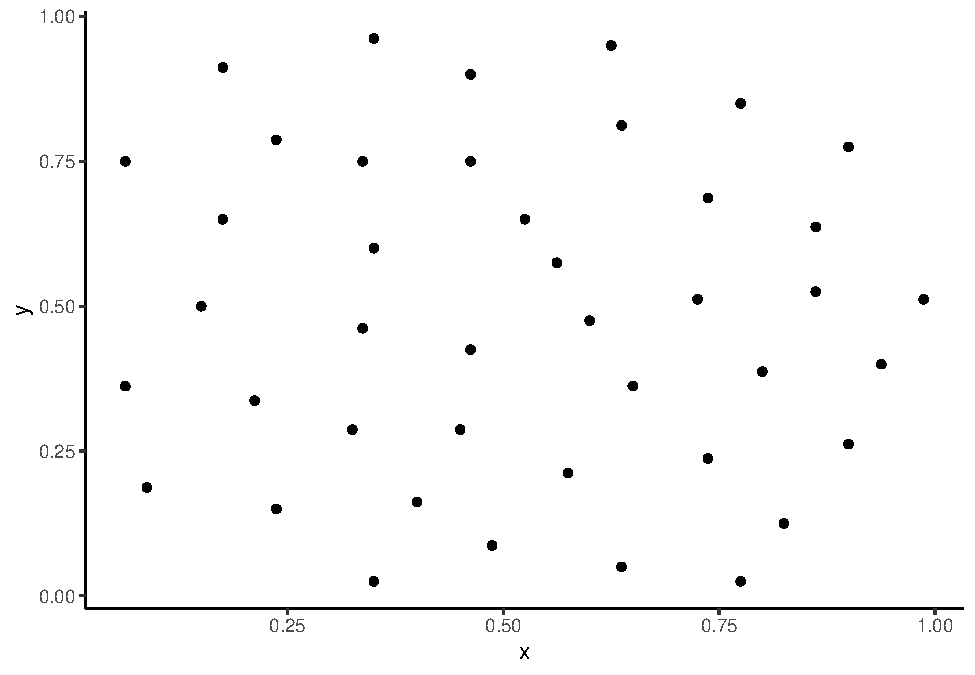
\includegraphics{project2_files/figure-latex/unnamed-chunk-19-1.pdf}
Seems to be evenly spread, no clear clusters. Look at \(J(t)\) plot

\begin{Shaded}
\begin{Highlighting}[]
\NormalTok{D =}\StringTok{ }\KeywordTok{ppregion}\NormalTok{(}\DataTypeTok{xl =} \DecValTok{0}\NormalTok{, }\DataTypeTok{xu =} \DecValTok{1}\NormalTok{, }\DataTypeTok{yl =} \DecValTok{0}\NormalTok{, }\DataTypeTok{yu =} \DecValTok{1}\NormalTok{)}

\NormalTok{cell.pp <-}\StringTok{ }\KeywordTok{list}\NormalTok{(}
  \DataTypeTok{x =}\NormalTok{ cell}\OperatorTok{$}\NormalTok{x, }
  \DataTypeTok{y =}\NormalTok{ cell}\OperatorTok{$}\NormalTok{y, }
  \DataTypeTok{area =}\NormalTok{ D}
\NormalTok{)}
\end{Highlighting}
\end{Shaded}

\begin{Shaded}
\begin{Highlighting}[]
\NormalTok{kfn.cell <-}\StringTok{ }\KeywordTok{Kfn}\NormalTok{(cell.pp, }\DecValTok{1}\NormalTok{, }\DataTypeTok{k =} \DecValTok{200}\NormalTok{)}
\KeywordTok{plot}\NormalTok{(kfn.cell)}
\end{Highlighting}
\end{Shaded}

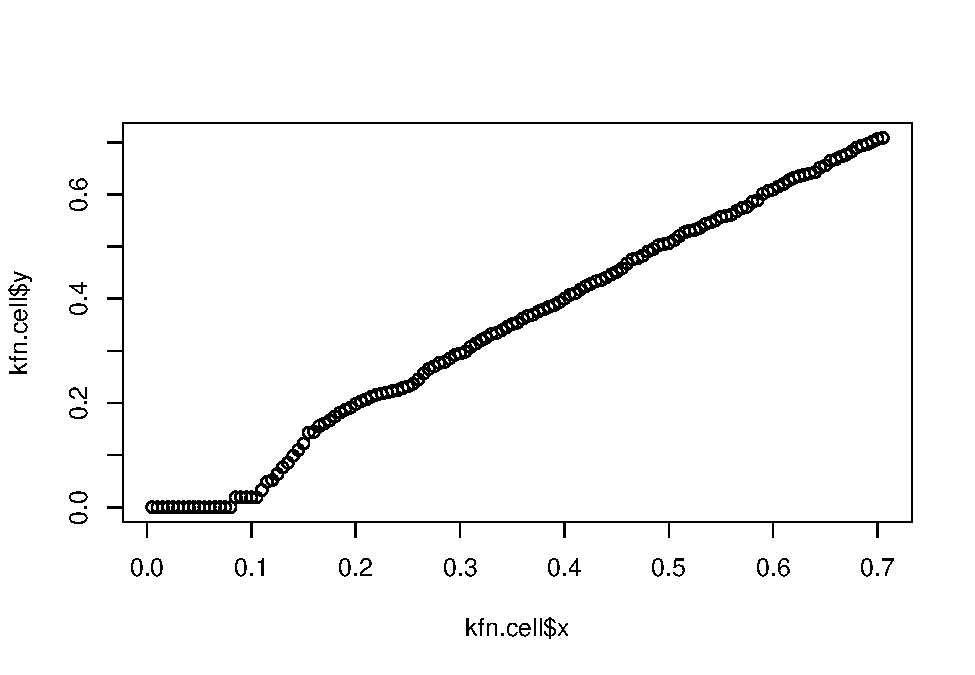
\includegraphics{project2_files/figure-latex/unnamed-chunk-21-1.pdf}

Calculating distances:

\begin{Shaded}
\begin{Highlighting}[]
\NormalTok{dist_mat <-}\StringTok{ }\KeywordTok{dist}\NormalTok{(cell, }\DataTypeTok{method =} \StringTok{'euclidean'}\NormalTok{) }\CommentTok{# Calculate distances}
\NormalTok{distances <-}\StringTok{ }\KeywordTok{as.vector}\NormalTok{(dist_mat)}
\end{Highlighting}
\end{Shaded}

Plotting distances:

\begin{Shaded}
\begin{Highlighting}[]
\KeywordTok{ggplot}\NormalTok{() }\OperatorTok{+}\StringTok{ }\KeywordTok{geom_density}\NormalTok{(}\KeywordTok{aes}\NormalTok{(}\DataTypeTok{x=}\NormalTok{distances), }\DataTypeTok{fill =} \StringTok{"skyblue"}\NormalTok{, }\DataTypeTok{alpha =} \FloatTok{0.5}\NormalTok{) }\OperatorTok{+}\StringTok{ }\KeywordTok{theme_classic}\NormalTok{() }\OperatorTok{+}\StringTok{ }\KeywordTok{xlab}\NormalTok{(}\StringTok{"Distance"}\NormalTok{) }\OperatorTok{+}\StringTok{ }\KeywordTok{ggtitle}\NormalTok{(}\StringTok{"Estiamted density of distance between points"}\NormalTok{)}
\end{Highlighting}
\end{Shaded}

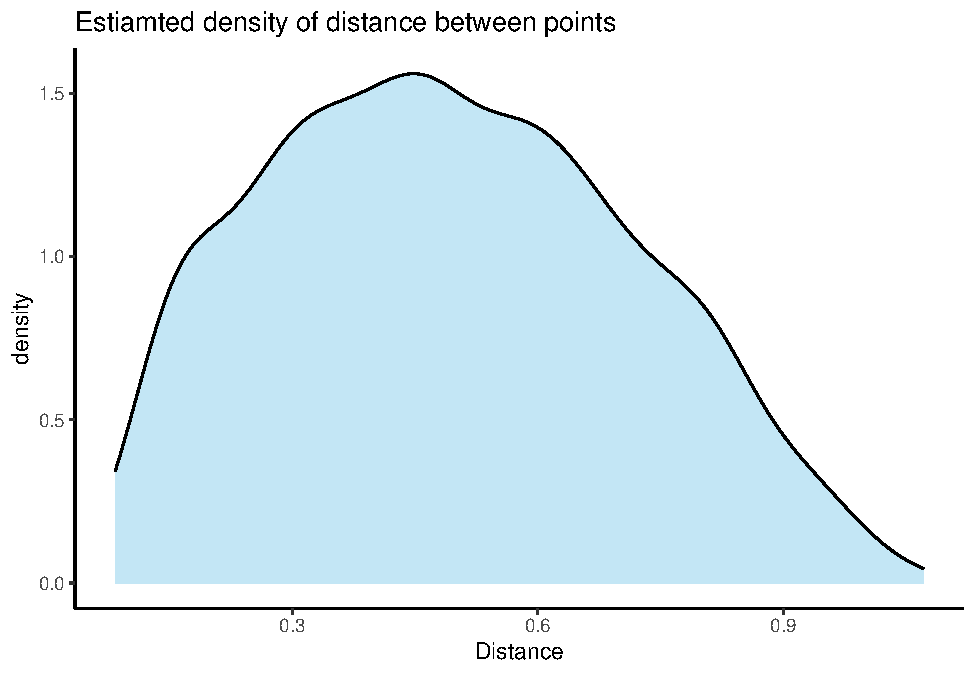
\includegraphics{project2_files/figure-latex/unnamed-chunk-23-1.pdf}

The minimum distance observed is 0.0836301. We set that to

\begin{Shaded}
\begin{Highlighting}[]
\KeywordTok{set.seed}\NormalTok{(}\DecValTok{2}\NormalTok{)}
\NormalTok{df <-}\StringTok{ }\NormalTok{cell}
\NormalTok{phi0 <-}\StringTok{ }\FloatTok{0.01}
\NormalTok{tau0 <-}\StringTok{ }\FloatTok{0.1} 
\NormalTok{phi1 <-}\StringTok{ }\DecValTok{1} 

\NormalTok{phi <-}\StringTok{ }\ControlFlowTok{function}\NormalTok{(tau, phi0, phi1, tau0)\{}
  \ControlFlowTok{if}\NormalTok{(tau }\OperatorTok{<}\StringTok{ }\NormalTok{tau0)\{}
\NormalTok{    phi0}
\NormalTok{  \}}
  
\NormalTok{  phi0}\OperatorTok{*}\KeywordTok{exp}\NormalTok{(}\OperatorTok{-}\NormalTok{phi1}\OperatorTok{*}\KeywordTok{abs}\NormalTok{(tau }\OperatorTok{-}\StringTok{ }\NormalTok{tau0))}
\NormalTok{\}}

\NormalTok{tau <-}\StringTok{ }\ControlFlowTok{function}\NormalTok{(x1, x2)\{}
  \KeywordTok{sqrt}\NormalTok{(}\KeywordTok{sum}\NormalTok{((x1}\OperatorTok{-}\NormalTok{x2)}\OperatorTok{^}\DecValTok{2}\NormalTok{)) }
\NormalTok{\}}

\NormalTok{gibsstep <-}\StringTok{ }\ControlFlowTok{function}\NormalTok{(df, phi0, tau0, phi1, }\DataTypeTok{all =}\NormalTok{ F)\{}
\NormalTok{  u <-}\StringTok{ }\KeywordTok{runif}\NormalTok{(}\KeywordTok{nrow}\NormalTok{(df))}
  
\NormalTok{  proposals <-}\StringTok{ }\NormalTok{df }
\NormalTok{  proposals}\OperatorTok{$}\NormalTok{accepted <-}\StringTok{ }\OtherTok{FALSE}
  
  \ControlFlowTok{for}\NormalTok{(i }\ControlFlowTok{in} \DecValTok{1}\OperatorTok{:}\KeywordTok{nrow}\NormalTok{(df))\{}
\NormalTok{    xu <-}\StringTok{ }\KeywordTok{as.vector}\NormalTok{(df[i,])}
\NormalTok{    xp <-}\StringTok{ }\KeywordTok{runif}\NormalTok{(}\DecValTok{2}\NormalTok{)}
    
\NormalTok{    right <-}\StringTok{ }\KeywordTok{apply}\NormalTok{(df, }\DecValTok{1}\NormalTok{, }\ControlFlowTok{function}\NormalTok{(x) }\KeywordTok{tau}\NormalTok{(xu, x))}
\NormalTok{    left <-}\StringTok{ }\KeywordTok{apply}\NormalTok{(df, }\DecValTok{1}\NormalTok{, }\ControlFlowTok{function}\NormalTok{(x) }\KeywordTok{tau}\NormalTok{(xp, x))}
    
\NormalTok{    right <-}\StringTok{ }\KeywordTok{sapply}\NormalTok{(right, }\ControlFlowTok{function}\NormalTok{(x) }\KeywordTok{phi}\NormalTok{(x, phi0, phi1, tau0))}
\NormalTok{    left <-}\StringTok{ }\KeywordTok{sapply}\NormalTok{(left, }\ControlFlowTok{function}\NormalTok{(x) }\KeywordTok{phi}\NormalTok{(x, phi0, phi1, tau0))}
    
\NormalTok{    res <-}\StringTok{ }\OperatorTok{-}\KeywordTok{sum}\NormalTok{(left }\OperatorTok{-}\StringTok{ }\NormalTok{right)}
\NormalTok{    alpha <-}\StringTok{ }\KeywordTok{exp}\NormalTok{(res)}
\NormalTok{    alpha <-}\StringTok{ }\KeywordTok{min}\NormalTok{(}\DecValTok{1}\NormalTok{, alpha)}
    \CommentTok{#print(alpha )}
    \ControlFlowTok{if}\NormalTok{(u[i] }\OperatorTok{<}\StringTok{ }\NormalTok{alpha)\{}
\NormalTok{      df[i,] =}\StringTok{ }\NormalTok{xp}
\NormalTok{      proposals[i,]}\OperatorTok{$}\NormalTok{accepted <-}\StringTok{ }\OtherTok{TRUE}

\NormalTok{    \}}
\NormalTok{    proposals[i,}\KeywordTok{c}\NormalTok{(}\DecValTok{1}\NormalTok{,}\DecValTok{2}\NormalTok{)] =}\StringTok{ }\NormalTok{xp}
\NormalTok{  \}}
  
  \ControlFlowTok{if}\NormalTok{(all)\{}
    \KeywordTok{return}\NormalTok{(}\KeywordTok{list}\NormalTok{(}\DataTypeTok{df =}\NormalTok{ df, }\DataTypeTok{proposals =}\NormalTok{ proposals))}
\NormalTok{  \}}
  
\NormalTok{  df}
\NormalTok{\}}
\end{Highlighting}
\end{Shaded}

\begin{Shaded}
\begin{Highlighting}[]
\NormalTok{df2 <-}\StringTok{ }\KeywordTok{gibsstep}\NormalTok{(df, phi0, tau0, phi1, }\DataTypeTok{all =}\NormalTok{ T)}\OperatorTok{$}\NormalTok{proposals}
\NormalTok{df.new <-}\StringTok{ }\KeywordTok{cbind}\NormalTok{(df, df2)}
\NormalTok{df.new}\OperatorTok{$}\NormalTok{id <-}\StringTok{ }\DecValTok{1}\OperatorTok{:}\KeywordTok{nrow}\NormalTok{(df.new)}
\KeywordTok{colnames}\NormalTok{(df.new) <-}\StringTok{ }\KeywordTok{c}\NormalTok{(}\StringTok{"x1"}\NormalTok{, }\StringTok{"y1"}\NormalTok{, }\StringTok{"x2"}\NormalTok{, }\StringTok{"y2"}\NormalTok{, }\StringTok{"accepted"}\NormalTok{,}\StringTok{"id"}\NormalTok{)}
\end{Highlighting}
\end{Shaded}

\begin{Shaded}
\begin{Highlighting}[]
\NormalTok{count =}\StringTok{ }\DecValTok{0}
\NormalTok{res <-}\StringTok{ }\KeywordTok{list}\NormalTok{()}
\NormalTok{df.t <-}\StringTok{ }\NormalTok{df}
\ControlFlowTok{while}\NormalTok{(count }\OperatorTok{<}\StringTok{ }\DecValTok{50}\NormalTok{)\{}
  \KeywordTok{print}\NormalTok{(count)}
\NormalTok{  df.t <-}\StringTok{ }\KeywordTok{gibsstep}\NormalTok{(df.t, phi0, tau0, phi1)}
\NormalTok{  count <-}\StringTok{ }\NormalTok{count }\OperatorTok{+}\StringTok{ }\DecValTok{1}
  \ControlFlowTok{if}\NormalTok{(count }\OperatorTok{==}\StringTok{ }\DecValTok{1}\NormalTok{)\{}
\NormalTok{    df}\FloatTok{.1}\NormalTok{ <-}\StringTok{ }\NormalTok{df.t}
\NormalTok{  \}}
  \CommentTok{#if(count > 20 && count %% 5 == 0)}
\NormalTok{  res <-}\StringTok{ }\KeywordTok{c}\NormalTok{(res, }\KeywordTok{list}\NormalTok{(df.t))}
\NormalTok{\}}
\end{Highlighting}
\end{Shaded}

\begin{verbatim}
## [1] 0
## [1] 1
## [1] 2
## [1] 3
## [1] 4
## [1] 5
## [1] 6
## [1] 7
## [1] 8
## [1] 9
## [1] 10
## [1] 11
## [1] 12
## [1] 13
## [1] 14
## [1] 15
## [1] 16
## [1] 17
## [1] 18
## [1] 19
## [1] 20
## [1] 21
## [1] 22
## [1] 23
## [1] 24
## [1] 25
## [1] 26
## [1] 27
## [1] 28
## [1] 29
## [1] 30
## [1] 31
## [1] 32
## [1] 33
## [1] 34
## [1] 35
## [1] 36
## [1] 37
## [1] 38
## [1] 39
## [1] 40
## [1] 41
## [1] 42
## [1] 43
## [1] 44
## [1] 45
## [1] 46
## [1] 47
## [1] 48
## [1] 49
\end{verbatim}

\begin{Shaded}
\begin{Highlighting}[]
\CommentTok{# Creating kfns}
\NormalTok{rels <-}\StringTok{ }\KeywordTok{lapply}\NormalTok{(res, }\ControlFlowTok{function}\NormalTok{(df) }\KeywordTok{list}\NormalTok{(}\DataTypeTok{x =}\NormalTok{ df[,}\DecValTok{1}\NormalTok{], }\DataTypeTok{y =}\NormalTok{ df[,}\DecValTok{2}\NormalTok{], }\DataTypeTok{area =}\NormalTok{ D))}
\NormalTok{kfns <-}\StringTok{ }\KeywordTok{lapply}\NormalTok{(rels, }\ControlFlowTok{function}\NormalTok{(rel) }\KeywordTok{Kfn}\NormalTok{(rel, }\DecValTok{1}\NormalTok{, }\DataTypeTok{k =} \DecValTok{200}\NormalTok{))}
\NormalTok{bands <-}\StringTok{ }\KeywordTok{sapply}\NormalTok{(kfns, }\ControlFlowTok{function}\NormalTok{(kfn) kfn}\OperatorTok{$}\NormalTok{y)}
\NormalTok{lower_band <-}\StringTok{ }\KeywordTok{apply}\NormalTok{(bands, }\DecValTok{1}\NormalTok{, }\ControlFlowTok{function}\NormalTok{(x) }\KeywordTok{quantile}\NormalTok{(x, }\DataTypeTok{probs =} \FloatTok{0.025}\NormalTok{))}
\NormalTok{upper_band <-}\StringTok{ }\KeywordTok{apply}\NormalTok{(bands, }\DecValTok{1}\NormalTok{, }\ControlFlowTok{function}\NormalTok{(x) }\KeywordTok{quantile}\NormalTok{(x, }\DataTypeTok{probs =} \FloatTok{0.975}\NormalTok{))}
\NormalTok{mid_band <-}\StringTok{ }\KeywordTok{apply}\NormalTok{(bands, }\DecValTok{1}\NormalTok{, }\ControlFlowTok{function}\NormalTok{(x) }\KeywordTok{quantile}\NormalTok{(x, }\DataTypeTok{probs =} \FloatTok{0.5}\NormalTok{))}
\end{Highlighting}
\end{Shaded}

Create trace plot

\begin{Shaded}
\begin{Highlighting}[]
\CommentTok{# x and y independent so look at trace for x and ys sepearetly. Look at poistion of first sel}
\NormalTok{pos1.x <-}\StringTok{ }\KeywordTok{sapply}\NormalTok{(res, }\ControlFlowTok{function}\NormalTok{(df) df[}\DecValTok{1}\NormalTok{,}\DecValTok{1}\NormalTok{])}
\NormalTok{pos1.y <-}\StringTok{ }\KeywordTok{sapply}\NormalTok{(res, }\ControlFlowTok{function}\NormalTok{(df) df[}\DecValTok{1}\NormalTok{,}\DecValTok{2}\NormalTok{])}

\CommentTok{# Create trace plots }
\KeywordTok{ggplot}\NormalTok{() }\OperatorTok{+}\StringTok{ }\KeywordTok{theme_classic}\NormalTok{() }\OperatorTok{+}\StringTok{ }\KeywordTok{geom_line}\NormalTok{(}\KeywordTok{aes}\NormalTok{(}\DataTypeTok{x =} \DecValTok{1}\OperatorTok{:}\KeywordTok{length}\NormalTok{(pos1.x), }\DataTypeTok{y =}\NormalTok{ pos1.x))}
\end{Highlighting}
\end{Shaded}

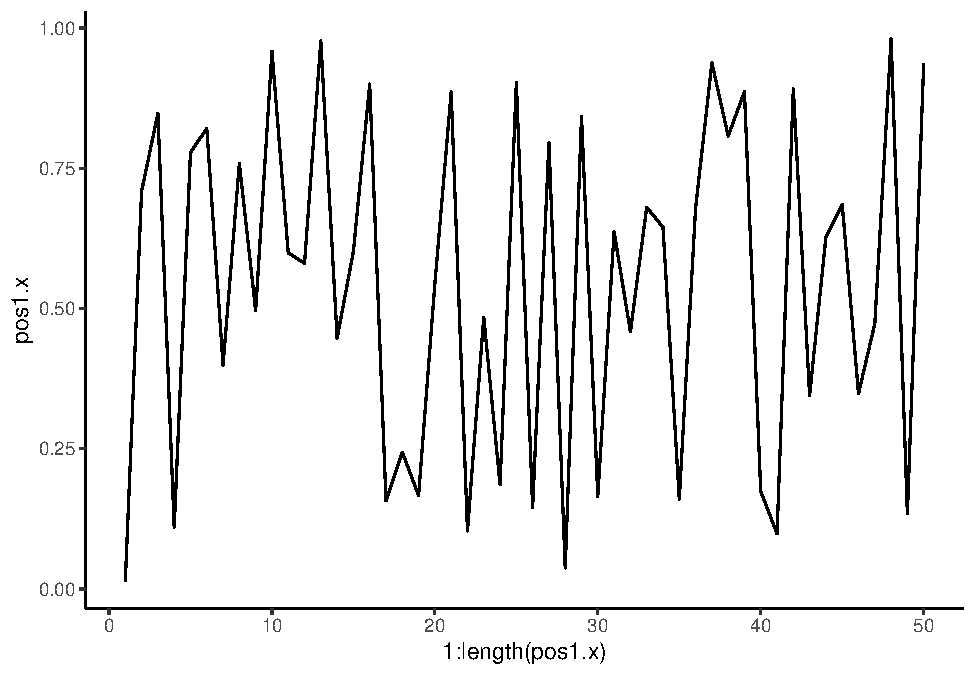
\includegraphics{project2_files/figure-latex/unnamed-chunk-27-1.pdf}

\begin{Shaded}
\begin{Highlighting}[]
\KeywordTok{ggplot}\NormalTok{() }\OperatorTok{+}\StringTok{ }\KeywordTok{theme_classic}\NormalTok{() }\OperatorTok{+}\StringTok{ }\KeywordTok{geom_line}\NormalTok{(}\KeywordTok{aes}\NormalTok{(}\DataTypeTok{x =} \DecValTok{1}\OperatorTok{:}\KeywordTok{length}\NormalTok{(pos1.y), }\DataTypeTok{y =}\NormalTok{ pos1.y))}
\end{Highlighting}
\end{Shaded}

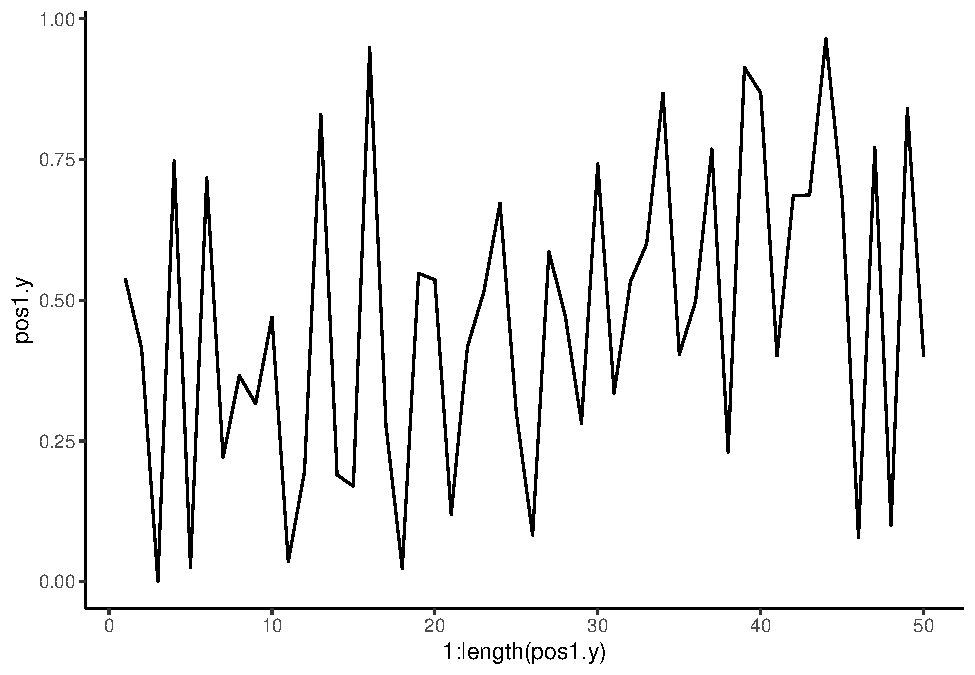
\includegraphics{project2_files/figure-latex/unnamed-chunk-27-2.pdf}

We first iteration, 5t iteration, 10th iteration and initial iteration
together

\begin{Shaded}
\begin{Highlighting}[]
\NormalTok{p0 <-}\StringTok{ }\KeywordTok{ggplot}\NormalTok{(}\DataTypeTok{data =}\NormalTok{ df) }\OperatorTok{+}\StringTok{ }\KeywordTok{geom_point}\NormalTok{(}\KeywordTok{aes}\NormalTok{(x,y)) }\OperatorTok{+}\StringTok{ }\KeywordTok{theme_classic}\NormalTok{() }\OperatorTok{+}\StringTok{ }\KeywordTok{ggtitle}\NormalTok{(}\StringTok{"Initial realization"}\NormalTok{)}
\NormalTok{p1 <-}\StringTok{ }\KeywordTok{ggplot}\NormalTok{(}\DataTypeTok{data =}\NormalTok{ df}\FloatTok{.1}\NormalTok{) }\OperatorTok{+}\StringTok{ }\KeywordTok{geom_point}\NormalTok{(}\KeywordTok{aes}\NormalTok{(x,y)) }\OperatorTok{+}\StringTok{ }\KeywordTok{theme_classic}\NormalTok{() }\OperatorTok{+}\StringTok{ }\KeywordTok{ggtitle}\NormalTok{(}\StringTok{"First realization"}\NormalTok{)}
\NormalTok{p2 <-}\StringTok{ }\KeywordTok{ggplot}\NormalTok{(}\DataTypeTok{data =}\NormalTok{ res[[}\DecValTok{1}\NormalTok{]]) }\OperatorTok{+}\StringTok{ }\KeywordTok{geom_point}\NormalTok{(}\KeywordTok{aes}\NormalTok{(x,y)) }\OperatorTok{+}\StringTok{ }\KeywordTok{theme_classic}\NormalTok{() }\OperatorTok{+}\StringTok{ }\KeywordTok{ggtitle}\NormalTok{(}\StringTok{"5th realization"}\NormalTok{)}
\NormalTok{p3 <-}\StringTok{ }\KeywordTok{ggplot}\NormalTok{(}\DataTypeTok{data =}\NormalTok{ res[[}\DecValTok{2}\NormalTok{]]) }\OperatorTok{+}\StringTok{ }\KeywordTok{geom_point}\NormalTok{(}\KeywordTok{aes}\NormalTok{(x,y)) }\OperatorTok{+}\StringTok{ }\KeywordTok{theme_classic}\NormalTok{() }\OperatorTok{+}\StringTok{ }\KeywordTok{ggtitle}\NormalTok{(}\StringTok{"10th realization"}\NormalTok{)}
\KeywordTok{ggarrange}\NormalTok{(p0, p1, p2, p3, }\DataTypeTok{nrow =} \DecValTok{2}\NormalTok{, }\DataTypeTok{ncol =} \DecValTok{2}\NormalTok{)}
\end{Highlighting}
\end{Shaded}

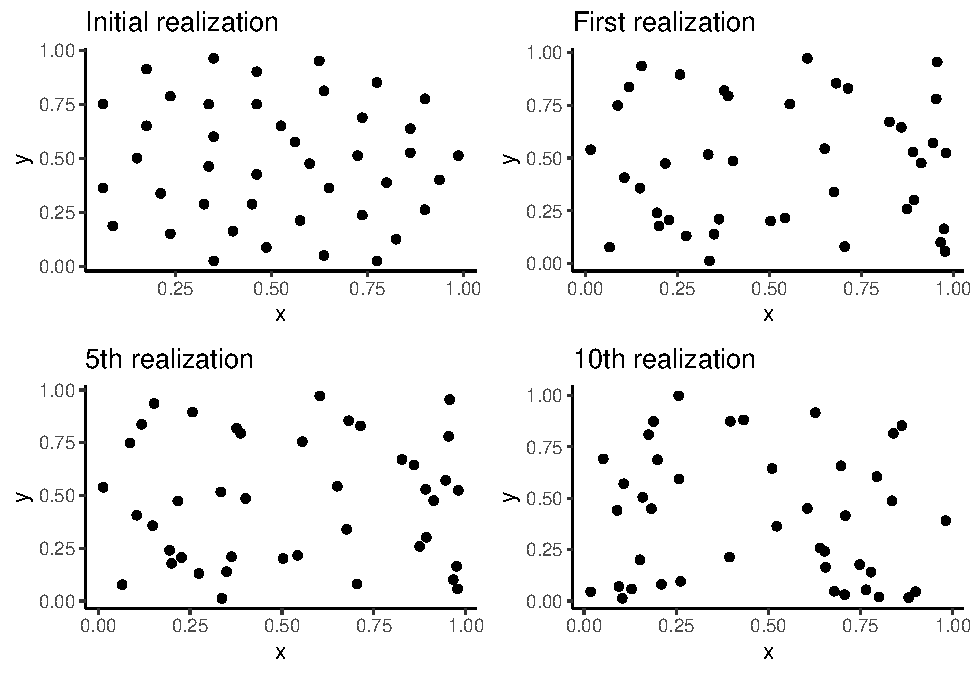
\includegraphics{project2_files/figure-latex/unnamed-chunk-28-1.pdf}

We plot a confidence band our simulated data and compare to the
observed.

\begin{Shaded}
\begin{Highlighting}[]
\KeywordTok{ggplot}\NormalTok{() }\OperatorTok{+}\StringTok{ }
\StringTok{  }\KeywordTok{geom_ribbon}\NormalTok{(}\KeywordTok{aes}\NormalTok{(}\DataTypeTok{x =}\NormalTok{ kfn.cell}\OperatorTok{$}\NormalTok{x, }\DataTypeTok{ymax =}\NormalTok{ upper_band, }\DataTypeTok{ymin =}\NormalTok{ lower_band), }\DataTypeTok{alpha =} \FloatTok{0.3}\NormalTok{) }\OperatorTok{+}
\StringTok{  }\KeywordTok{geom_line}\NormalTok{(}\KeywordTok{aes}\NormalTok{(}\DataTypeTok{x =}\NormalTok{ kfn.cell}\OperatorTok{$}\NormalTok{x, }\DataTypeTok{y =}\NormalTok{ kfn.cell}\OperatorTok{$}\NormalTok{y)) }\OperatorTok{+}
\StringTok{  }\KeywordTok{theme_classic}\NormalTok{()}
\end{Highlighting}
\end{Shaded}

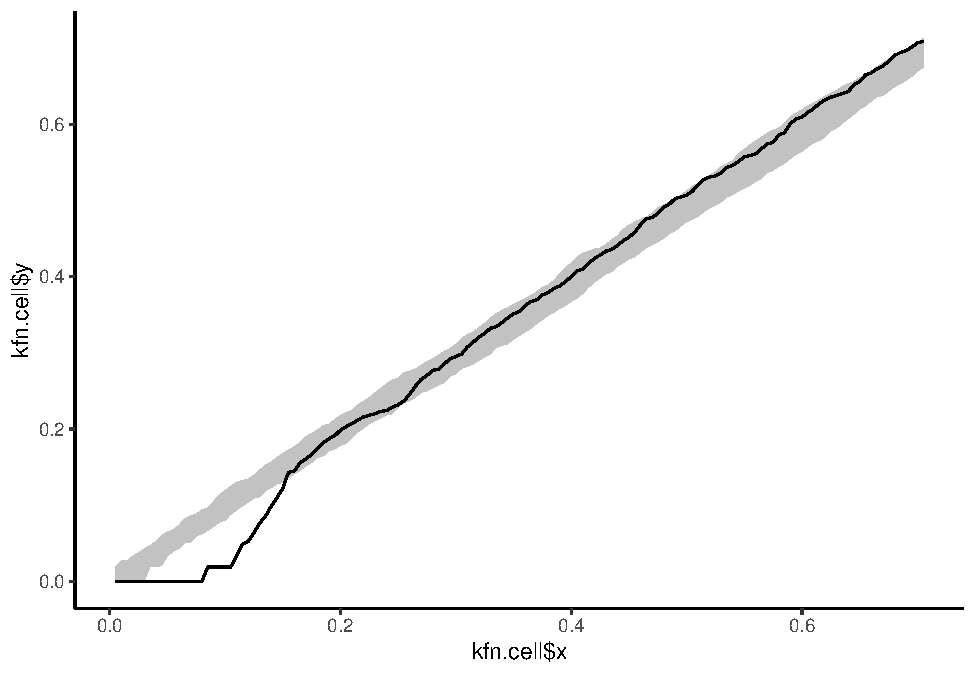
\includegraphics{project2_files/figure-latex/unnamed-chunk-29-1.pdf}

We see that we miss on cells that are close, thus decide to increase
\(\phi0\) in hopes of it giving a better fit.

\begin{Shaded}
\begin{Highlighting}[]
\KeywordTok{set.seed}\NormalTok{(}\DecValTok{2}\NormalTok{)}
\NormalTok{df <-}\StringTok{ }\NormalTok{cell}
\NormalTok{phi0 <-}\StringTok{ }\FloatTok{0.1}
\NormalTok{tau0 <-}\StringTok{ }\FloatTok{0.1} 
\NormalTok{phi1 <-}\StringTok{ }\DecValTok{1} 
\end{Highlighting}
\end{Shaded}

\end{document}
